%%%%%%%%%%%%%%%%%%%%%%%%%%%%%%%%%%%%%%%%%
% 
% This template is adapted from Mathias Legrand's and Vel's
% "Orange Book" template v2.4, licensed under CC BY-NC-SA 3.0
% (http://creativecommons.org/licenses/by-nc-sa/3.0/)

% Compiling requires to run:
%
% 1) pdflatex main
% 2) makeindex main.idx -s StyleInd.ist
% 3) biber main
% 4) pdflatex main x 2
%
% Important note:
% Chapter heading images should have a 2:1 width:height ratio,
% e.g. 920px width and 460px height.
%
%%%%%%%%%%%%%%%%%%%%%%%%%%%%%%%%%%%%%%%%%

\documentclass[11pt,fleqn]{book} % Default font size and left-justified equations

%%%%%%%%%%%%%%%%%%%%%%%%%%%%%%%%%%%%%%%%%
% The Legrand Orange Book
% Structural Definitions File
% Version 2.1 (26/09/2018)
%
% Original author:
% Mathias Legrand (legrand.mathias@gmail.com) with modifications by:
% Vel (vel@latextemplates.com)
%
% This file was downloaded from:
% http://www.LaTeXTemplates.com
%
% License:
% CC BY-NC-SA 3.0 (http://creativecommons.org/licenses/by-nc-sa/3.0/)
%
%%%%%%%%%%%%%%%%%%%%%%%%%%%%%%%%%%%%%%%%%

%----------------------------------------------------------------------------------------
%	VARIOUS REQUIRED PACKAGES AND CONFIGURATIONS
%----------------------------------------------------------------------------------------

\usepackage{graphicx} % Required for including pictures
\graphicspath{{Pictures/}} % Specifies the directory where pictures are stored

\usepackage{lipsum} % Inserts dummy text

\usepackage{tikz} % Required for drawing custom shapes

\usepackage[english]{babel} % English language/hyphenation

\usepackage{enumitem} % Customize lists
\setlist{nolistsep} % Reduce spacing between bullet points and numbered lists

\usepackage{booktabs} % Required for nicer horizontal rules in tables

\usepackage{xcolor} % Required for specifying colors by name
\definecolor{ocre}{RGB}{243,102,25} % Define the orange color used for highlighting throughout the book

%----------------------------------------------------------------------------------------
%	MARGINS
%----------------------------------------------------------------------------------------

\usepackage{geometry} % Required for adjusting page dimensions and margins

\geometry{
	paper=a4paper, % Paper size, change to letterpaper for US letter size
	top=3cm, % Top margin
	bottom=3cm, % Bottom margin
	left=3cm, % Left margin
	right=3cm, % Right margin
	headheight=14pt, % Header height
	footskip=1.4cm, % Space from the bottom margin to the baseline of the footer
	headsep=10pt, % Space from the top margin to the baseline of the header
	%showframe, % Uncomment to show how the type block is set on the page
}

%----------------------------------------------------------------------------------------
%	FONTS
%----------------------------------------------------------------------------------------

\usepackage{avant} % Use the Avantgarde font for headings
%\usepackage{times} % Use the Times font for headings
\usepackage{mathptmx} % Use the Adobe Times Roman as the default text font together with math symbols from the Sym­bol, Chancery and Com­puter Modern fonts

\usepackage{microtype} % Slightly tweak font spacing for aesthetics
\usepackage[utf8]{inputenc} % Required for including letters with accents
\usepackage[T1]{fontenc} % Use 8-bit encoding that has 256 glyphs

%----------------------------------------------------------------------------------------
%	BIBLIOGRAPHY AND INDEX
%----------------------------------------------------------------------------------------

\usepackage[natbib=true,citestyle=authoryear,sorting=nyt,sortcites=true,autopunct=true,babel=hyphen,hyperref=true,abbreviate=false,backref=true,backend=biber]{biblatex}
\addbibresource{stats.bib} % BibTeX bibliography file
\addbibresource{learning.bib} % BibTeX bibliography file
\defbibheading{bibempty}{}

\usepackage{calc} % For simpler calculation - used for spacing the index letter headings correctly
\usepackage{makeidx} % Required to make an index
\makeindex % Tells LaTeX to create the files required for indexing

%----------------------------------------------------------------------------------------
%	MAIN TABLE OF CONTENTS
%----------------------------------------------------------------------------------------

\usepackage{titletoc} % Required for manipulating the table of contents

\contentsmargin{0cm} % Removes the default margin

% Part text styling (this is mostly taken care of in the PART HEADINGS section of this file)
\titlecontents{part}
	[0cm] % Left indentation
	{\addvspace{20pt}\bfseries} % Spacing and font options for parts
	{}
	{}
	{}

% Chapter text styling
\titlecontents{chapter}
	[1.25cm] % Left indentation
	{\addvspace{12pt}\large\sffamily\bfseries} % Spacing and font options for chapters
	{\color{ocre!60}\contentslabel[\Large\thecontentslabel]{1.25cm}\color{ocre}} % Formatting of numbered sections of this type
	{\color{ocre}} % Formatting of numberless sections of this type
	{\color{ocre!60}\normalsize\;\titlerule*[.5pc]{.}\;\thecontentspage} % Formatting of the filler to the right of the heading and the page number

% Section text styling
\titlecontents{section}
	[1.25cm] % Left indentation
	{\addvspace{3pt}\sffamily\bfseries} % Spacing and font options for sections
	{\contentslabel[\thecontentslabel]{1.25cm}} % Formatting of numbered sections of this type
	{} % Formatting of numberless sections of this type
	{\hfill\color{black}\thecontentspage} % Formatting of the filler to the right of the heading and the page number

% Subsection text styling
\titlecontents{subsection}
	[1.25cm] % Left indentation
	{\addvspace{1pt}\sffamily\small} % Spacing and font options for subsections
	{\contentslabel[\thecontentslabel]{1.25cm}} % Formatting of numbered sections of this type
	{} % Formatting of numberless sections of this type
	{\ \titlerule*[.5pc]{.}\;\thecontentspage} % Formatting of the filler to the right of the heading and the page number

% Figure text styling
\titlecontents{figure}
	[1.25cm] % Left indentation
	{\addvspace{1pt}\sffamily\small} % Spacing and font options for figures
	{\thecontentslabel\hspace*{1em}} % Formatting of numbered sections of this type
	{} % Formatting of numberless sections of this type
	{\ \titlerule*[.5pc]{.}\;\thecontentspage} % Formatting of the filler to the right of the heading and the page number

% Table text styling
\titlecontents{table}
	[1.25cm] % Left indentation
	{\addvspace{1pt}\sffamily\small} % Spacing and font options for tables
	{\thecontentslabel\hspace*{1em}} % Formatting of numbered sections of this type
	{} % Formatting of numberless sections of this type
	{\ \titlerule*[.5pc]{.}\;\thecontentspage} % Formatting of the filler to the right of the heading and the page number

%----------------------------------------------------------------------------------------
%	MINI TABLE OF CONTENTS IN PART HEADS
%----------------------------------------------------------------------------------------

% Chapter text styling
\titlecontents{lchapter}
	[0em] % Left indentation
	{\addvspace{15pt}\large\sffamily\bfseries} % Spacing and font options for chapters
	{\color{ocre}\contentslabel[\Large\thecontentslabel]{1.25cm}\color{ocre}} % Chapter number
	{}
	{\color{ocre}\normalsize\sffamily\bfseries\;\titlerule*[.5pc]{.}\;\thecontentspage} % Page number

% Section text styling
\titlecontents{lsection}
	[0em] % Left indentation
	{\sffamily\small} % Spacing and font options for sections
	{\contentslabel[\thecontentslabel]{1.25cm}} % Section number
	{}
	{}

% Subsection text styling (note these aren't shown by default, display them by searchings this file for tocdepth and reading the commented text)
\titlecontents{lsubsection}
	[.5em] % Left indentation
	{\sffamily\footnotesize} % Spacing and font options for subsections
	{\contentslabel[\thecontentslabel]{1.25cm}}
	{}
	{}

%----------------------------------------------------------------------------------------
%	HEADERS AND FOOTERS
%----------------------------------------------------------------------------------------

\usepackage{fancyhdr} % Required for header and footer configuration

\pagestyle{fancy} % Enable the custom headers and footers

\renewcommand{\chaptermark}[1]{\markboth{\sffamily\normalsize\bfseries\chaptername\ \thechapter.\ #1}{}} % Styling for the current chapter in the header
\renewcommand{\sectionmark}[1]{\markright{\sffamily\normalsize\thesection\hspace{5pt}#1}{}} % Styling for the current section in the header

\fancyhf{} % Clear default headers and footers
\fancyhead[LE,RO]{\sffamily\normalsize\thepage} % Styling for the page number in the header
\fancyhead[LO]{\rightmark} % Print the nearest section name on the left side of odd pages
\fancyhead[RE]{\leftmark} % Print the current chapter name on the right side of even pages
%\fancyfoot[C]{\thepage} % Uncomment to include a footer

\renewcommand{\headrulewidth}{0.5pt} % Thickness of the rule under the header

\fancypagestyle{plain}{% Style for when a plain pagestyle is specified
	\fancyhead{}\renewcommand{\headrulewidth}{0pt}%
}

% Removes the header from odd empty pages at the end of chapters
\makeatletter
\renewcommand{\cleardoublepage}{
\clearpage\ifodd\c@page\else
\hbox{}
\vspace*{\fill}
\thispagestyle{empty}
\newpage
\fi}

%----------------------------------------------------------------------------------------
%	THEOREM STYLES
%----------------------------------------------------------------------------------------

\usepackage{amsmath,amsfonts,amssymb,amsthm} % For math equations, theorems, symbols, etc
\usepackage{bbm} % for mathbbm
\newtheorem{lemma}{Lemma}
\newcommand{\intoo}[2]{\mathopen{]}#1\,;#2\mathclose{[}}
\newcommand{\ud}{\mathop{\mathrm{{}d}}\mathopen{}}
\newcommand{\intff}[2]{\mathopen{[}#1\,;#2\mathclose{]}}
\renewcommand{\qedsymbol}{$\blacksquare$}
\newtheorem{notation}{Notation}[chapter]

% Boxed/framed environments
\newtheoremstyle{ocrenumbox}% Theorem style name
{0pt}% Space above
{0pt}% Space below
{\normalfont}% Body font
{}% Indent amount
{\small\bf\sffamily\color{ocre}}% Theorem head font
{\;}% Punctuation after theorem head
{0.25em}% Space after theorem head
{\small\sffamily\color{ocre}\thmname{#1}\nobreakspace\thmnumber{\@ifnotempty{#1}{}\@upn{#2}}% Theorem text (e.g. Theorem 2.1)
\thmnote{\nobreakspace\the\thm@notefont\sffamily\bfseries\color{black}---\nobreakspace#3.}} % Optional theorem note

\newtheoremstyle{blacknumex}% Theorem style name
{5pt}% Space above
{5pt}% Space below
{\normalfont}% Body font
{} % Indent amount
{\small\bf\sffamily}% Theorem head font
{\;}% Punctuation after theorem head
{0.25em}% Space after theorem head
{\small\sffamily{\tiny\ensuremath{\blacksquare}}\nobreakspace\thmname{#1}\nobreakspace\thmnumber{\@ifnotempty{#1}{}\@upn{#2}}% Theorem text (e.g. Theorem 2.1)
\thmnote{\nobreakspace\the\thm@notefont\sffamily\bfseries---\nobreakspace#3.}}% Optional theorem note

\newtheoremstyle{blacknumbox} % Theorem style name
{0pt}% Space above
{0pt}% Space below
{\normalfont}% Body font
{}% Indent amount
{\small\bf\sffamily}% Theorem head font
{\;}% Punctuation after theorem head
{0.25em}% Space after theorem head
{\small\sffamily\thmname{#1}\nobreakspace\thmnumber{\@ifnotempty{#1}{}\@upn{#2}}% Theorem text (e.g. Theorem 2.1)
\thmnote{\nobreakspace\the\thm@notefont\sffamily\bfseries---\nobreakspace#3.}}% Optional theorem note

% Non-boxed/non-framed environments
\newtheoremstyle{ocrenum}% Theorem style name
{5pt}% Space above
{5pt}% Space below
{\normalfont}% Body font
{}% Indent amount
{\small\bf\sffamily\color{ocre}}% Theorem head font
{\;}% Punctuation after theorem head
{0.25em}% Space after theorem head
{\small\sffamily\color{ocre}\thmname{#1}\nobreakspace\thmnumber{\@ifnotempty{#1}{}\@upn{#2}}% Theorem text (e.g. Theorem 2.1)
\thmnote{\nobreakspace\the\thm@notefont\sffamily\bfseries\color{black}---\nobreakspace#3.}} % Optional theorem note
\makeatother

% Defines the theorem text style for each type of theorem to one of the three styles above
\newcounter{dummy}
\numberwithin{dummy}{section}
\theoremstyle{ocrenumbox}
\newtheorem{theoremeT}[dummy]{Theorem}
\newtheorem{problem}{Problem}[chapter]
\newtheorem{exerciseT}{Exercise}[chapter]
\theoremstyle{blacknumex}
\newtheorem{exampleT}{Example}[chapter]
\theoremstyle{blacknumbox}
\newtheorem{vocabulary}{Vocabulary}[chapter]
\newtheorem{definitionT}{Definition}[section]
\newtheorem{corollaryT}[dummy]{Corollary}
\theoremstyle{ocrenum}
\newtheorem{proposition}[dummy]{Proposition}

%----------------------------------------------------------------------------------------
%	DEFINITION OF COLORED BOXES
%----------------------------------------------------------------------------------------

\RequirePackage[framemethod=default]{mdframed} % Required for creating the theorem, definition, exercise and corollary boxes

% Theorem box
\newmdenv[skipabove=7pt,
skipbelow=7pt,
backgroundcolor=black!5,
linecolor=ocre,
innerleftmargin=5pt,
innerrightmargin=5pt,
innertopmargin=5pt,
leftmargin=0cm,
rightmargin=0cm,
innerbottommargin=5pt]{tBox}

% Exercise box
\newmdenv[skipabove=7pt,
skipbelow=7pt,
rightline=false,
leftline=true,
topline=false,
bottomline=false,
backgroundcolor=ocre!10,
linecolor=ocre,
innerleftmargin=5pt,
innerrightmargin=5pt,
innertopmargin=5pt,
innerbottommargin=5pt,
leftmargin=0cm,
rightmargin=0cm,
linewidth=4pt]{eBox}

% Definition box
\newmdenv[skipabove=7pt,
skipbelow=7pt,
rightline=false,
leftline=true,
topline=false,
bottomline=false,
linecolor=ocre,
innerleftmargin=5pt,
innerrightmargin=5pt,
innertopmargin=0pt,
leftmargin=0cm,
rightmargin=0cm,
linewidth=4pt,
innerbottommargin=0pt]{dBox}

% Corollary box
\newmdenv[skipabove=7pt,
skipbelow=7pt,
rightline=false,
leftline=true,
topline=false,
bottomline=false,
linecolor=gray,
backgroundcolor=black!5,
innerleftmargin=5pt,
innerrightmargin=5pt,
innertopmargin=5pt,
leftmargin=0cm,
rightmargin=0cm,
linewidth=4pt,
innerbottommargin=5pt]{cBox}

% Creates an environment for each type of theorem and assigns it a theorem text style from the "Theorem Styles" section above and a colored box from above
\newenvironment{theorem}{\begin{tBox}\begin{theoremeT}}{\end{theoremeT}\end{tBox}}
\newenvironment{exercise}{\begin{eBox}\begin{exerciseT}}{\hfill{\color{ocre}\tiny\ensuremath{\blacksquare}}\end{exerciseT}\end{eBox}}
\newenvironment{definition}{\begin{dBox}\begin{definitionT}}{\end{definitionT}\end{dBox}}
\newenvironment{example}{\begin{exampleT}}{\hfill{\tiny\ensuremath{\blacksquare}}\end{exampleT}}
\newenvironment{corollary}{\begin{cBox}\begin{corollaryT}}{\end{corollaryT}\end{cBox}}

%----------------------------------------------------------------------------------------
%	REMARK ENVIRONMENT
%----------------------------------------------------------------------------------------

\newenvironment{remark}{\par\vspace{10pt}\small % Vertical white space above the remark and smaller font size
\begin{list}{}{
\leftmargin=35pt % Indentation on the left
\rightmargin=25pt}\item\ignorespaces % Indentation on the right
\makebox[-2.5pt]{\begin{tikzpicture}[overlay]
\node[draw=ocre!60,line width=1pt,circle,fill=ocre!25,font=\sffamily\bfseries,inner sep=2pt,outer sep=0pt] at (-15pt,0pt){\textcolor{ocre}{R}};\end{tikzpicture}} % Orange R in a circle
\advance\baselineskip -1pt}{\end{list}\vskip5pt} % Tighter line spacing and white space after remark

%----------------------------------------------------------------------------------------
%	SECTION NUMBERING IN THE MARGIN
%----------------------------------------------------------------------------------------

\makeatletter
\renewcommand{\@seccntformat}[1]{\llap{\textcolor{ocre}{\csname the#1\endcsname}\hspace{1em}}}
\renewcommand{\section}{\@startsection{section}{1}{\z@}
{-4ex \@plus -1ex \@minus -.4ex}
{1ex \@plus.2ex }
{\normalfont\large\sffamily\bfseries}}
\renewcommand{\subsection}{\@startsection {subsection}{2}{\z@}
{-3ex \@plus -0.1ex \@minus -.4ex}
{0.5ex \@plus.2ex }
{\normalfont\sffamily\bfseries}}
\renewcommand{\subsubsection}{\@startsection {subsubsection}{3}{\z@}
{-2ex \@plus -0.1ex \@minus -.2ex}
{.2ex \@plus.2ex }
{\normalfont\small\sffamily\bfseries}}
\renewcommand\paragraph{\@startsection{paragraph}{4}{\z@}
{-2ex \@plus-.2ex \@minus .2ex}
{.1ex}
{\normalfont\small\sffamily\bfseries}}

%----------------------------------------------------------------------------------------
%	PART HEADINGS
%----------------------------------------------------------------------------------------

% Numbered part in the table of contents
\newcommand{\@mypartnumtocformat}[2]{%
	\setlength\fboxsep{0pt}%
	\noindent\colorbox{ocre!20}{\strut\parbox[c][.7cm]{\ecart}{\color{ocre!70}\Large\sffamily\bfseries\centering#1}}\hskip\esp\colorbox{ocre!40}{\strut\parbox[c][.7cm]{\linewidth-\ecart-\esp}{\Large\sffamily\centering#2}}%
}

% Unnumbered part in the table of contents
\newcommand{\@myparttocformat}[1]{%
	\setlength\fboxsep{0pt}%
	\noindent\colorbox{ocre!40}{\strut\parbox[c][.7cm]{\linewidth}{\Large\sffamily\centering#1}}%
}

\newlength\esp
\setlength\esp{4pt}
\newlength\ecart
\setlength\ecart{1.2cm-\esp}
\newcommand{\thepartimage}{}%
\newcommand{\partimage}[1]{\renewcommand{\thepartimage}{#1}}%
\def\@part[#1]#2{%
\ifnum \c@secnumdepth >-2\relax%
\refstepcounter{part}%
\addcontentsline{toc}{part}{\texorpdfstring{\protect\@mypartnumtocformat{\thepart}{#1}}{\partname~\thepart\ ---\ #1}}
\else%
\addcontentsline{toc}{part}{\texorpdfstring{\protect\@myparttocformat{#1}}{#1}}%
\fi%
\startcontents%
\markboth{}{}%
{\thispagestyle{empty}%
\begin{tikzpicture}[remember picture,overlay]%
\node at (current page.north west){\begin{tikzpicture}[remember picture,overlay]%
\fill[ocre!20](0cm,0cm) rectangle (\paperwidth,-\paperheight);
\node[anchor=north] at (4cm,-3.25cm){\color{ocre!40}\fontsize{220}{100}\sffamily\bfseries\thepart};
\node[anchor=south east] at (\paperwidth-1cm,-\paperheight+1cm){\parbox[t][][t]{8.5cm}{
\printcontents{l}{0}{\setcounter{tocdepth}{1}}% The depth to which the Part mini table of contents displays headings; 0 for chapters only, 1 for chapters and sections and 2 for chapters, sections and subsections
}};
\node[anchor=north east] at (\paperwidth-1.5cm,-3.25cm){\parbox[t][][t]{15cm}{\strut\raggedleft\color{white}\fontsize{30}{30}\sffamily\bfseries#2}};
\end{tikzpicture}};
\end{tikzpicture}}%
\@endpart}
\def\@spart#1{%
\startcontents%
\phantomsection
{\thispagestyle{empty}%
\begin{tikzpicture}[remember picture,overlay]%
\node at (current page.north west){\begin{tikzpicture}[remember picture,overlay]%
\fill[ocre!20](0cm,0cm) rectangle (\paperwidth,-\paperheight);
\node[anchor=north east] at (\paperwidth-1.5cm,-3.25cm){\parbox[t][][t]{15cm}{\strut\raggedleft\color{white}\fontsize{30}{30}\sffamily\bfseries#1}};
\end{tikzpicture}};
\end{tikzpicture}}
\addcontentsline{toc}{part}{\texorpdfstring{%
\setlength\fboxsep{0pt}%
\noindent\protect\colorbox{ocre!40}{\strut\protect\parbox[c][.7cm]{\linewidth}{\Large\sffamily\protect\centering #1\quad\mbox{}}}}{#1}}%
\@endpart}
\def\@endpart{\vfil\newpage
\if@twoside
\if@openright
\null
\thispagestyle{empty}%
\newpage
\fi
\fi
\if@tempswa
\twocolumn
\fi}

%----------------------------------------------------------------------------------------
%	CHAPTER HEADINGS
%----------------------------------------------------------------------------------------

% A switch to conditionally include a picture, implemented by Christian Hupfer
\newif\ifusechapterimage
\usechapterimagetrue
\newcommand{\thechapterimage}{}%
\newcommand{\chapterimage}[1]{\ifusechapterimage\renewcommand{\thechapterimage}{#1}\fi}%
\newcommand{\autodot}{.}
\def\@makechapterhead#1{%
{\parindent \z@ \raggedright \normalfont
\ifnum \c@secnumdepth >\m@ne
\if@mainmatter
\begin{tikzpicture}[remember picture,overlay]
\node at (current page.north west)
{\begin{tikzpicture}[remember picture,overlay]
\node[anchor=north west,inner sep=0pt] at (0,0) {\ifusechapterimage\includegraphics[width=\paperwidth]{\thechapterimage}\fi};
\draw[anchor=west] (\Gm@lmargin,-9cm) node [line width=2pt,rounded corners=15pt,draw=ocre,fill=white,fill opacity=0.5,inner sep=15pt]{\strut\makebox[22cm]{}};
\draw[anchor=west] (\Gm@lmargin+.3cm,-9cm) node {\huge\sffamily\bfseries\color{black}\thechapter\autodot~#1\strut};
\end{tikzpicture}};
\end{tikzpicture}
\else
\begin{tikzpicture}[remember picture,overlay]
\node at (current page.north west)
{\begin{tikzpicture}[remember picture,overlay]
\node[anchor=north west,inner sep=0pt] at (0,0) {\ifusechapterimage\includegraphics[width=\paperwidth]{\thechapterimage}\fi};
\draw[anchor=west] (\Gm@lmargin,-9cm) node [line width=2pt,rounded corners=15pt,draw=ocre,fill=white,fill opacity=0.5,inner sep=15pt]{\strut\makebox[22cm]{}};
\draw[anchor=west] (\Gm@lmargin+.3cm,-9cm) node {\huge\sffamily\bfseries\color{black}#1\strut};
\end{tikzpicture}};
\end{tikzpicture}
\fi\fi\par\vspace*{270\p@}}}

%-------------------------------------------

\def\@makeschapterhead#1{%
\begin{tikzpicture}[remember picture,overlay]
\node at (current page.north west)
{\begin{tikzpicture}[remember picture,overlay]
\node[anchor=north west,inner sep=0pt] at (0,0) {\ifusechapterimage\includegraphics[width=\paperwidth]{\thechapterimage}\fi};
\draw[anchor=west] (\Gm@lmargin,-9cm) node [line width=2pt,rounded corners=15pt,draw=ocre,fill=white,fill opacity=0.5,inner sep=15pt]{\strut\makebox[22cm]{}};
\draw[anchor=west] (\Gm@lmargin+.3cm,-9cm) node {\huge\sffamily\bfseries\color{black}#1\strut};
\end{tikzpicture}};
\end{tikzpicture}
\par\vspace*{270\p@}}
\makeatother

%----------------------------------------------------------------------------------------
%	LINKS
%----------------------------------------------------------------------------------------

\usepackage{hyperref}
\hypersetup{hidelinks,backref=true,pagebackref=true,hyperindex=true,colorlinks=true,citecolor=blue,breaklinks=true,urlcolor=ocre,bookmarks=true,bookmarksopen=false}

\usepackage{bookmark}
\bookmarksetup{
open,
numbered,
addtohook={%
\ifnum\bookmarkget{level}=0 % chapter
\bookmarksetup{bold}%
\fi
\ifnum\bookmarkget{level}=-1 % part
\bookmarksetup{color=ocre,bold}%
\fi
}
}

\newcommand\un[1]{\textcolor{magenta}{#1}}
\newcommand\unn[1]{\textcolor{blue}{#1}}
\newcommand\unnn[1]{\textcolor{red}{#1}}
\newcommand\unnnn[1]{\textcolor{orange}{#1}}

\def\cX{\mathcal{X}}
\def\cY{\mathcal{Y}}
\def\cZ{\mathcal{Z}}
\def\cS{\mathcal{S}}
\def\cR{\mathcal{R}}
\def\cA{\mathcal{A}}

\def\by{\mathbf{y}}

% indicator
\newcommand\IND[1]{\mathbbm{1}_{\{#1\}}}

\def\cfdemo{\url{https://chi-feng.github.io/mcmc-demo/}}

\def\tpi{\widetilde{\pi}}
\def\cN{\mathcal{N}}
\renewcommand\d{\mathrm{d}}
\def\e{\mathrm{e}}

%\hypersetup{pdftitle={Title},pdfauthor={Author}} % Uncomment and fill out to include PDF metadata for the author and title of the book

\begin{document}
\begingroup
    \thispagestyle{empty} % Suppress headers and footers on the title page
    \begin{tikzpicture}[remember picture,overlay]
        \node[inner sep=0pt] (background) at (current page.center) {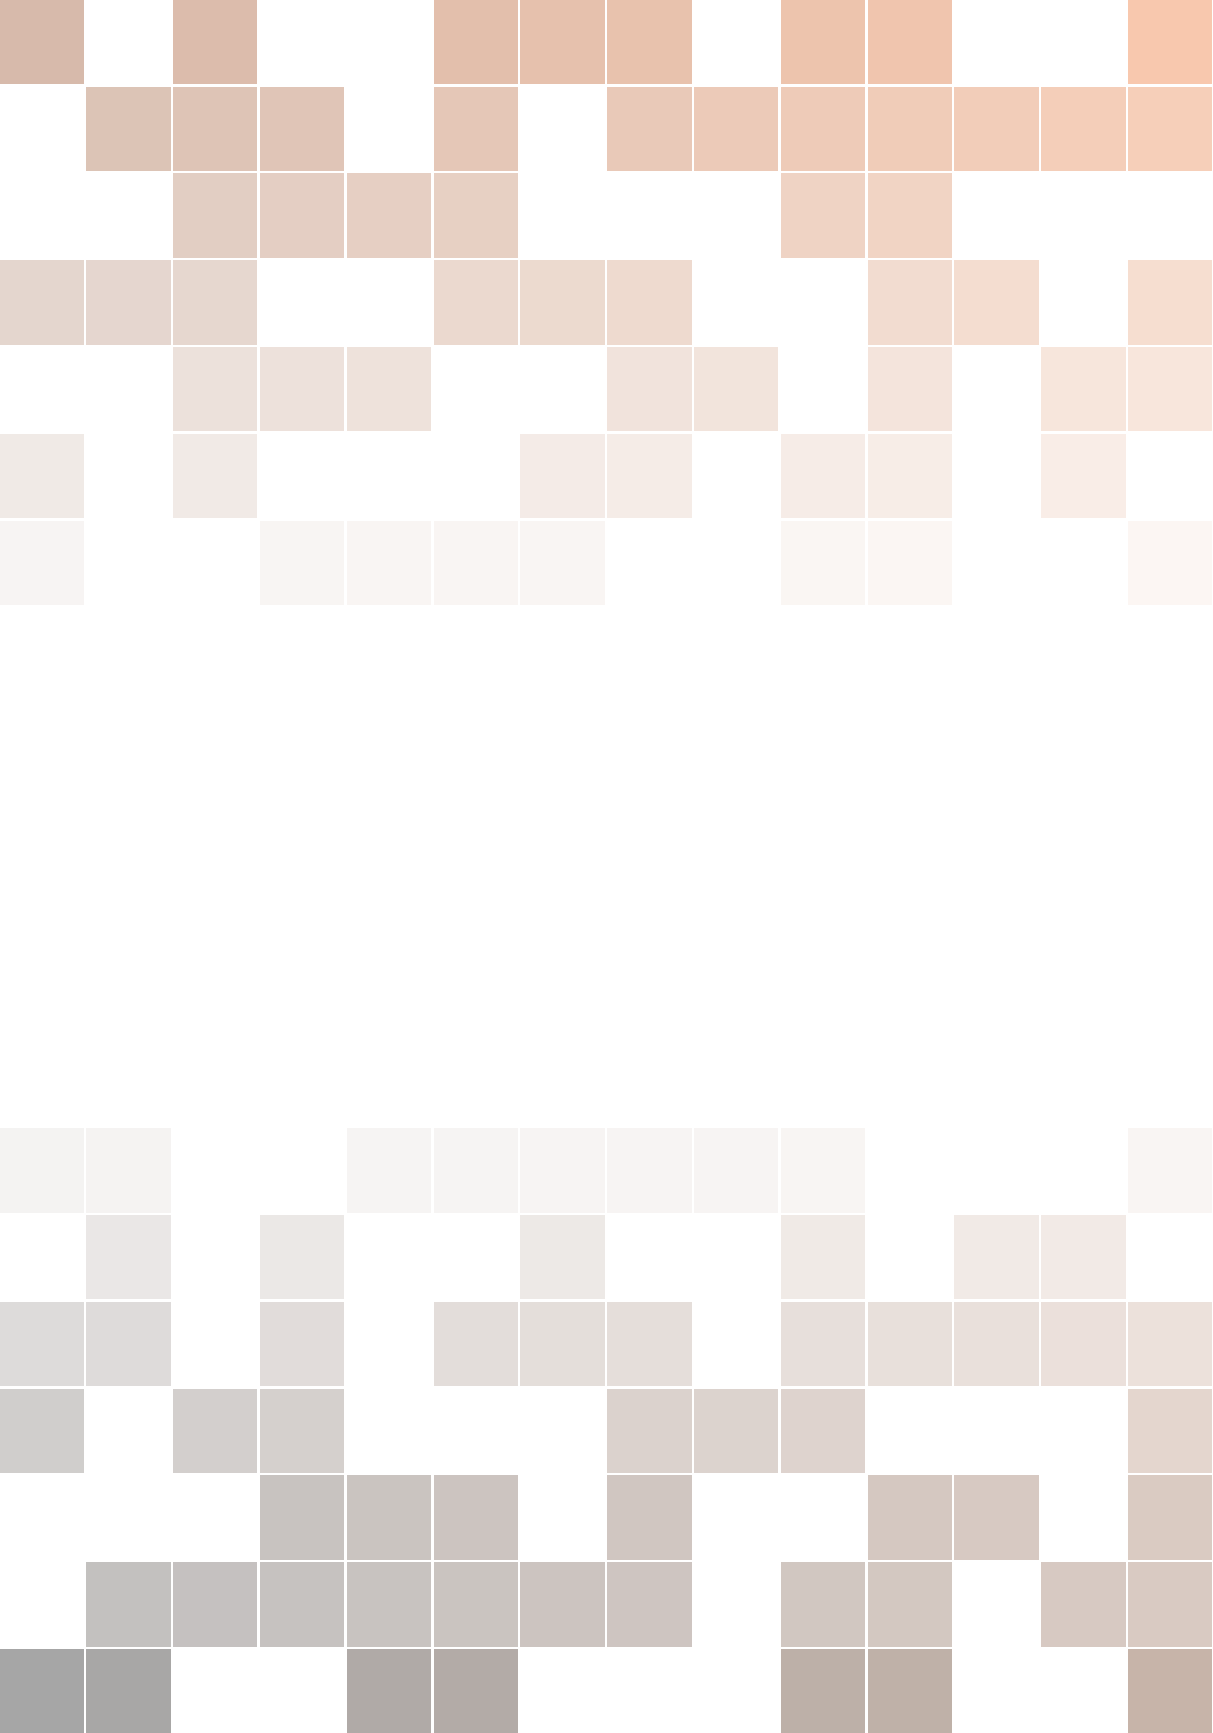
\includegraphics[width=\paperwidth]{background.pdf}};
        \draw (current page.center) node [fill=ocre!30!white,fill opacity=0.6,text opacity=1,inner sep=1cm]{\Huge\centering\bfseries\sffamily\parbox[c][][t]{\paperwidth}{\centering Lecture notes on Bayesian machine learning\\[15pt] % Book title
        {\Large What is BML, why use it, and how to implement it.}\\[20pt] % Subtitle
        {\huge R\'emi Bardenet}}}; % Author name
    \end{tikzpicture}

    \vfill
\endgroup


%----------------------------------------------------------------------------------------
%	COPYRIGHT PAGE
%----------------------------------------------------------------------------------------

\newpage
~\vfill
\thispagestyle{empty}

\noindent Copyright \copyright\ 2021 Rémi Bardenet and Julyan Arbel\\ % Copyright notice

%\noindent \textsc{Published by Publisher}\\ % Publisher
% \noindent \textsc{book-website.com}\\ % URL

\noindent This template is adapted from Mathias Legrand's and Vel's
 \emph{Orange Book} template v2.4, licensed under CC BY-NC-SA 3.0
 (\url{http://creativecommons.org/licenses/by-nc-sa/3.0/}).

%----------------------------------------------------------------------------------------
%	TABLE OF CONTENTS
%----------------------------------------------------------------------------------------

%\usechapterimagefalse % If you don't want to include a chapter image, use this to toggle images off - it can be enabled later with \usechapterimagetrue

\chapterimage{chapter_head_1.pdf} % Table of contents heading image
\pagestyle{empty} % Disable headers and footers for the following pages
\tableofcontents % Print the table of contents itself
\cleardoublepage % Forces the first chapter to start on an odd page so it's on the right side of the book
\pagestyle{fancy} % Enable headers and footers again

\part{What is Bayesian machine learning?}
    \chapterimage{chapter_head_2.pdf} % Chapter heading image
    \chapter{The example of penalized linear regression}
    \label{ch:penalized_linear_regression}
    In this chapter, we introduce different historical approaches to learning and inference on a running example, penalized linear regression. 
We shall exagerate the stances of some famous scientists, for the sake of illustration. 

\section{Fisher does linear regression}

Say we have a data set $(x_i,y_i)$, $1\leq i\leq N$, where $x_i\in\mathbb{R}^d$ are the \emph{features} and $y_i\in\mathbb{R}$ the \emph{response}. 
We want to study the influence of features on the response, and we ask British statistician Ronald Fisher (1890--1962) for help. 
He recommends positing a simple statistical model, i.e. a parametrized collection of PDFs for $y\vert x$. 
Calling the parameter $\theta$ and abusively denoting the parametrized distributions by $y\vert x,\theta$, we posit 
$$ p(y_i\vert x_i, \theta) = \cN(y_i \vert x_i^T \theta, \sigma^2), 1\leq i \leq N,$$
i.i.d., with known $\sigma$ for simplicity.
To characterize the influence of features on the response, Fisher recommends that we estimate $\theta$, along with a confidence interval to communicate our uncertainty. 
Fisher was the one to introduce the maximum likelihood estimator 
$$
\tMLE \triangleq \arg\max_{\theta} p(\by\vert X, \theta) = \arg\max_\theta \prod_{i=1}^N \cN(y_i \vert x_i^T \theta, \sigma^2).
$$
Now 
$$
\log \prod_{i=1}^N \cN(y_i \vert x_i^T \theta, \sigma^2) = \log \cN(\by \vert X\theta, \sigma^2 I) \propto - \Vert \by - X\theta\Vert^2,
$$
where the proportionality sign allows us to drop additive terms that do not depend on $\theta$. 
This entails that $\tMLE$ is nothing but the least squares estimator 
$$
\tMLE = (X^TX)^{-1} X^T\by,
$$
where we assumed that $X$ has full rank.
There is nothing inherently good in using the MLE rather than another estimator, but it often has good \emph{frequentist} properties, i.e., properties established by integrating over the posited data generation model.
For instance, it is easy to prove the following.
\begin{proposition}
Under $\by \sim \cN(X\theta, \sigma^2 I)$, and assuming $X$ has full rank,
\begin{equation}
    \label{e:fisher}
    \tMLE \sim \cN(\theta, \sigma^2(X^TX)^{-1}).
\end{equation}
\end{proposition}
\proofLeftAsExercise

Fisher then argues that \eqref{e:fisher} gives you a wealth of properties that make $\tMLE$ an interesting estimator.
For starters, $\tMLE$ is unbiased ($\mathbb E \tMLE = \theta$)
and $\tMLE \rightarrow \theta$ in probability. 
Moreover, the (random) ellipsoid 
$$
\mathcal{E}_\alpha = \{\theta\in\mathbb{R}^d \text{ such that }\sigma^{-2}(\theta-\tMLE)^TX^T X(\theta-\tMLE) \leq \alpha\} 
$$
contains $\theta$ with known probability $1-\delta(\alpha)$.
It thus makes sense, to Fisher, to find the smallest value $\alpha_{0.99}$ such that $1-\delta(\alpha)\geq 0.99$, and report the \emph{confidence region} $\mathcal{E}_{\alpha_0.99}$ to quantify his uncertainty about $\theta$. 
The fact that, under repetition of the data generation, the (random) ellipsoid $\mathcal{E}_{\alpha_0.99}$ contains $\theta$ about $99\%$ of the time, is called \emph{coverage}.

\section{Wald does linear regression}
Imagine that you had asked Hungarian-American Abraham Wald (1902--1950) for help instead of Fisher.
He would have argued that estimating $\theta$, or outputing a region of $\mathbb{R}^d$ that encodes your uncertainty, are two different actions to be taken under uncertainty. 

Consider estimation. 
Wald would ask you to specify the loss $L(\theta,\widehat{\theta})$ that you incur by estimating $\theta$ by $\widehat{\theta}\in\mathbb{R}^d$. 
You might answer $L_\alpha(\theta,\widehat{\theta}) = \Vert\theta-\widehat{\theta}\Vert^\alpha$ for some $\alpha>0$.
Wald would then say that the accuracy of an estimator $\widehat{\theta}= \widehat{\theta}(\by)$ is characterized by its risk function
\begin{equation}
    R(\cdot,\widehat{\theta}):\theta\mapsto \mathbb{E}_{\by\vert X, \theta} L(\theta,\widehat{\theta}(\by)).
    \label{e:risk}
\end{equation}
If the risk function of an estimator is smaller than that of another estimator, we say that the former dominates the latter.
Wald's minimum requirement for an estimator is that the estimator is \emph{admissible}, i.e., that it is not dominated. 
Maybe surprisingly, the MLE for regression with the squared loss $L_2$ is \emph{not} admissible! 
This is an extension by \cite{TBC} of an important theorem known as the James-Stein theorem \citep{TBC}.
We leave the original James-Stein theorem as \exo{ex:james-stein}. 
We shall see an even simpler estimator that dominates the MLE in Section~\ref{s:ridge_regression}.

So what should we do, according to Wald, if the MLE is no option? 
It would be natural to find an estimator with as small as possible a risk function.
Unfortunately, the risk function being a function, many pairs of estimators are incomparable. 
Wald might recommend to sum up a risk function by a single number, and look, for instance, for an estimator minimizing the worst-case risk, a so-called \emph{minimax} estimator
\begin{equation}
    \widehat\theta_{\text{minimax}} \in \arg\inf_{\widehat{\theta}} \sup_\theta R(\theta,\widehat{\theta}).
    \label{e:minimax_estimator_for_regression}
\end{equation}
Another solution to sum up the risk function is to integrate it against a measure for which the risk is integrable. 
This leads to an estimator that we call the \emph{Bayes} estimator, anticipating over Chapter~\ref{ch:expected_utility},
\begin{equation}
    \tBayes \in \arg\min_{\widehat{\theta}} \mathbb{E}_\theta R(\theta,\widehat{\theta}) = \mathbb{E}_\theta \mathbb{E}_{\by\vert X,\theta} R(\theta,\widehat{\theta}).
    \label{e:bayes_estimator_for_regression}
\end{equation}
We now have a joint distribution over $\theta,\by$. 
As long as the loss $L(\theta,\widehat{\theta}(\by))$ is integratble w.r.t. this joint, the towering property of the expectation yields
\begin{align}
    \mathbb{E}_\theta \mathbb{E}_{\by\vert X,\theta} L(\theta,\widehat{\theta}) 
    &= \mathbb{E}_\by \mathbb{E}_{\theta\vert X,\by} L(\theta,\widehat{\theta}).
\label{e:reversed_expectation}
\end{align}
Since $\widehat{\theta}$ is only a function $\by$, minimizing \eqref{e:reversed_expectation} boils down to setting 
$$
\tBayes = \tBayes(\by) = \arg\inf_{\widehat{\theta}} \mathbb{E}_{\theta\vert X,\by} L(\theta,\widehat{\theta}).
$$
For the squared loss $L=L_2$, the Bayes estimator is thus the mean of the \emph{posterior} distribution, i.e. 
$
\mathbb{E}_{\theta\vert X,\by} \theta. 
$
For the one-loss $L=L_1$, the Bayes estimator is a generalized median of the same posterior distribution.

\section{Savage does linear regression}
\label{ch:bayesian_regression}
% introduce subjective Bayes

\section{Hoerl and Kennard do linear regression}
\label{ch:penalized_regression}
% introduce empirical Bayes

    \chapter{Maximizing expected utility}
    \label{ch:expected_utility}
    After formally defining decision problems, we show that basic machine learning problems such as classification, regression, model choice, etc. are decision problems. 
Then we introduce subjective expected utility, the single unique guideline of all Bayesians, and go over its consequences for ML decisions.
Justifying subjective expected utility shall wait until Chapter~\ref{ch:foundations}.

For this chapter, I mostly used two references.
\citep{PaIn09} focuses on ideas and is a formidable entry point to (Bayesian) decision theory, while \citep{Sch11} is a great textbook-level reference for mathematical details.

\section{Decision problem}

Formally, a decision problem is defined as 
\begin{enumerate}
    \item a set $\cS$ of \emph{states}. For technical reasons, we also require a $\sigma$-algebra $\Sigma_\cS$ that makes $(\cS, \Sigma_\cS)$ a Borel space \citep{Sch11}.
    \item a set of \emph{rewards} $\cR$. We also require a $\sigma$-algebra $\Sigma_R$, which should contain all singletons. 
    \item a set $\cA$ of measurable functions from $\cS$ to $\cR$, called \emph{actions}.
\end{enumerate}
We think of states as encoding all information about the situation at hand. Actions are what we are tasked to choose, and picking action $a$ while the situation is described by a given state $s$ leads to reward $a(s)$.
Note\footnote{In future versions of the course, we might make the framework more general, to include, e.g. Markov decision processes.} that we assume here that the same set of actions $\cA$ remains available in every state $s$.

    %\section{Lists}\index{Lists}
    %\subsection{Numbered List}\index{Lists!Numbered List}

\part{Foundations}
    \label{ch:foundations}
    \chapterimage{chapter_head_1.pdf} % Chapter heading image
    \chapter{Many (incompatible) reasons to be a Bayesian}
    %!TEX root = ./main.tex
So far, the main appeal of subjective expected utility (SEU) has been its conceptual simplicity, and the fact that it answers all decision problems in the same manner. 
In this chapter, we review some attempts at justifying SEU more formally, i.e. show that SEU logically follows from some simple, consensual principle.
When you hear someone say that ``Non-Bayesians are incoherent'', that ``a prior encapsulates the information available \emph{before} an experiment is made, so that the prior cannot depend on data", or that ``the posterior is the experimenter's updated belief after the experiment", or that ``Non-Bayesians violate the likelihood principle", they are all referring to one or the other of the formal justifications below. 
Not all these justifications are compatible, and none can really claim to be uniformly superior, so it is important to know upon what arguments you are resting your interpretation of the Bayesian procedure.

\section{Because you abide by the likelihood principle}
The ``formal" likelihood principle \citep{BeWo88} is a half-formal justification that deals primarily with the estimation problem. 
It is only half-formal because it deals with notions that are hard to rigorously define.

\subsection{The formal LP}
Consider two statistical experiments
$$
E_i=(\cY_i,\un{s}, \{p_i(\cdot\vert\vartheta), \vartheta\in\Theta\}), \quad i=1,2.
$$
Assume that for some realizations $\by_1$ and $\by_2$,
$$
p_1(\by_1\vert\cdot) \propto p_2(\by_2\vert \cdot).
$$
Note that we are using bold characters to insist on $\by_1$ and $\by_2$ being vectors concatenating (possibly many, of arbitrary dimension) observations, the label $i=1,2$ is only there to indicate which experiment we consider.
In particular, $\by_1$ and $\by_2$ may differ in dimension.

Now, assuming that there exists a quantity $\text{Ev}(E,x)$ that encapsulates the ``evidence on $\theta$ arising from $E$ and $x$", the formal LP principle is the requirement that
$$
\text{Ev}(E_1,\by_1) = \text{Ev}(E_2,\by_2).
$$
As a corollary, $\text{Ev}(E,\by)$ can depend on $x$ solely through $p(\by\vert\cdot)$.

\subsection{SEU satisfies the LP}
Letting $\cS = \cY^n\times\theta$, SEU satisfies the LP as long as the joint distribution over states has either $p_1$ or $p_2$ as its conditional of $\by$ given $\theta$.
Indeed, let
$$
p_i(s_i) = p_i(\by_i,\theta) = p_i(\by_i\vert\theta)\un{p(\theta)} = \un{Z} p_i(\theta\vert \by_i), \quad i=1,2.
$$
Note how we use a common prior. 
Then for $a:\cS\rightarrow\cZ$,
  $$ 
  \int L(a,s_1) \frac{p_1(\by_1\vert\theta)p(\theta)}{\un{Z}} \d\theta \propto \int L(a,s_2) \frac{p_2(\by_2\vert\theta)p(\theta)}{\un{Z}} \d\theta, 
  $$
  so that the posterior expected losses are the same in both experiments, and Bayes actions coincide.
  However, note that full expected utilities are different in general, 
  \begin{align*}
    \int L(a,s_1) p_1(\by_1\vert\theta)p(\theta) \unn{\d \by_1}\d\theta
    &\neq \int L(a,s_2) p_2(\by_2\vert\theta)p(\theta) \unn{\d \by_2}\d\theta.
  \end{align*}

\subsection{The stopping rule principle}
The same kind of computations shows that SEU with a particular choice of joint distribution is immune to data-dependent stopping rules. 
This can also be seen as a consequence of the LP \citep{BeWo88}, but we stick to SEU with some conditions on its joint distribution of states for simplicity.

Assume that we want to model the following inference problem.
We collect data one item at a time, independently from some distribution $y_i\vert\theta$, until the first $n\in\mathbb{N}$ such that $y_1,\dots,y_n \in A_n$, and then you want to estimate $\theta$. 
We model this by $\cS = \Theta \times \cup_{n\geq 1} \cY^n$, and decide to take a joint distribution $p$  such that $y_1,y_2,\dots$ are independent given $\theta$, just like we assume the data generating mechanism works. 
Then the Bayes action $a^\star = a_{g^\star}$ minimizes
\begin{align*}
   \mathbb E L(a,s) &= \mathbb E \left [ L(a,s) \sum_{n} \un{\IND{N=n}} \right ]\\
    &= \sum_{n} \mathbb E \left [ L(a,s) \un{\IND{N=N}} \right ]\\
    &= \sum_{n} \int L(a,(\theta,y_{1:n})) \un{\IND{y_{1:n}\in A_n}\prod_{k<n}\IND{y_{1:k}\notin A_k}} p(y_{1:n}\vert\theta) p(\theta) \d y_{1:n}\d \theta.\\
    &= \sum_n \int\d y_{1:n} \un{\IND{y_{1:n}\in A_n}\prod_{k<n}\IND{y_{1:k} \notin A_k}} \int  L(a,(\theta,y_{1:n}))  p(y_{1:n}\vert\theta) p(\theta),
\end{align*}
where we used the monotone convergence theorem and Fubini's theorem (assuming, e.g., that the loss is bounded).
So, to find the minimizer $g^\star$ defined on $\cup_n \cY^n$ of the overall expected loss, it is enough, for each $n$, to define $g^\star(y_{1:n})$ as the usual Bayes rule for fixed $n$, i.e. as the minimizer of the inner integral.
In other words, as long as the prior $p(\theta)$ does not depend on data, the Bayes decision is immune to data-dependent stopping rules: just act as if there were no stopping rule.

\subsection{Pros and cons of the LP}
\begin{itemize}
  \item The LP is compelling to many \citep{BeWo88}, but it has its downsides.
  \item Being Bayesian is not the only way to abide by the LP.
  \item I am personally uncomfortable with the stopping rule principle, probably because my frequentist intuition is still too strong.
  \item It is hard to make fully formal: is $\text{Ev}(E,x)$ even meaningful? See answer by LeCam to \citep{BeWo88}.
  \item It assumes we want to specify a likelihood, this prevents model-free Bayesianism.
  \item It separates the roles of the likelihood and the prior. For LP-abiding Bayesians, \un{the prior is not allowed to depend on data}.
\end{itemize}

% % ###############################################
\section{Because you place coherence above all things: subjective Bayes}
The literature on the foundations of subjective Bayes is rich, and we refer to \citep{PaIn09} for entry points. 
A major milestone was obtained by \cite{Sav53}, building on work of \cite{VoMo} and \cite{Ram}. 
Savage gave a list of properties (the so-called \emph{Savage axioms} of coherence) that a binary relation $\succ$ on the action space $\cA$ should satisfy in order for it to have an essentially unique expected utility representation.
More precisely, $\succ$ satisfies the Savage axioms if and only if there is a bounded utility function $u:\mathcal{S}\rightarrow\mathcal{R}_+$ and a (finitely additive) probability measure $p$ on $\mathcal{S}$ such that for $a, b\in \mathcal{A}$, 
$$
a \succ b \Leftrightarrow \int u(a(s))\d p(s) > \int u(b(s))\d p(s);
$$
$u$ is unique up to affine transformations. 
The pair $(u,p)$ thus characterizes the behaviour of a Savage-abiding decision maker, whose preferred action is the one minimizing the expected utility. 
This is the sense of the word \emph{subjective} in SEU: the probability $p$, as well as the utility $u$, live in the mind of the DM. 
This is also the sense in which $p$ can be interpreted as the DM's degree of belief.
Finally, note that there is no constraint on the probability $p$: any pair $(u,p)$ corresponds to a coherent decision-maker. 
In other words, Savage tells you that to be coherent you have to follow SEU, but it does not help you choose a joint model over states, let alone a prior.

Savage's result is beautiful, in that it builds a probability measure $p$ and a utility function $u$ over states from a coherent ranking of actions.
Following Savage, there is no need to assume that the phenomenon we are studying is probabilistic, or to dissentangle different forms of uncertainty: a coherent decision maker \emph{must} have a utility and a probability in mind!
We now take a closer look at Savage's axioms as an example of prescritive subjective Bayesian framework, and examine some common criticisms.

\subsection{A closer look at the axioms}
% \cite{Sav54} derives a unique (finitely additive) probability on $2^\cS$ and utility function directly from a preference relation over acts $a:\cS\rightarrow\cZ$. He relies on NM, but without compound acts (considered as artificial) and no physical chance mechanism (unlike Ramsey or Anscombe \& Aumann).
Since axiom numbers `Px' in the original paper of \cite{Sav54} are often referred to as such, I use them as labels. Yet I introduce axioms in the same order as \cite{PaIn09}.

An important thing to notice before looking at his axioms, is that Savage considers the action set $\cA$ to be all functions from $\cS$ to $\cZ$. 
In particular, constant actions, i.e. actions of the type $s\mapsto z$ for some $z\in\cZ$, play a crucial role in Savage's derivation, even if they do not correspond to actual actions available to the decision maker (DM) in most cases. 
In the sequel, we abusively denote by $z$ the constant action $s\mapsto z$.

\begin{axiom}{P1 (Preference)}\label{a:P1}
$\succ$ is complete and transitive.
\end{axiom}

Since $\succ$ is complete, we can thus check whether $z_1\succ z_2$ for any two constant actions $z_1,z_2$.

\begin{axiom}{P5 (No total indifference)}\label{a:P5}
$\exists z_1,z_2\in\cZ$ such that $z_1\succ z_2$.
\end{axiom}
\begin{example}
  \label{e:binary_classification}
  If we take binary classification as a running example, where $\cZ=\{0,1\}$, the only two constant actions are the ``ideal" classifier $0$ that is always right and the one that is always wrong.
  Most of us will likely elicit $0\succ 1$, to say that we prefer being always right to being always wrong.
  Note that none of the two constant actions usually belong to the "pratically accessible" actions $\{a_g:s \mapsto y - g(x; x_{1:n}, y_{1:n}), g\in \mathcal{G}\}$.
\end{example}

Now for $a,b\in\cA$, $T\in\cS$, define action $a_{T}^b$ by $a_{T}^b(s) = a(s)1_{s\in T} + b(s)1_{s\in T}$.

\begin{axiom}{P2 (Sure Thing principle)}\label{a:P2}
$\forall a,b,h_1,h_2\in\cA$ and $\forall T\subset\cS$,
$$ a_{T^c}^{h_1} \succ b_{T^c}^{h_1} \Leftrightarrow a_{T^c}^{h_2} \succ b_{T^c}^{h_2}.$$
\end{axiom}
% Axiom~\ref{a:P2} is similar to \ref{a:NM2}, but doesn't use compound acts. 
Here, Savage directly formulates that if two acts coincide on part of $\cS$, then preference should only depend on their values where they differ. 
In particular, under \ref{a:P2}, we can define a new family of preference relations, called \emph{conditional preferences}.
Let $T\subset\cS$, and define $a\succ b\vert T$ by
\begin{equation}
c_{T}^a \succ c_T^b
\label{e:conditionalPreference}
\end{equation}
for some (equivalently all) $c\in \cA$. 
This family of conditional preferences will be discussed later, when we consider how to rank actions after some $T$ has been observed.
\begin{example}[Continuation of Example~\ref{e:binary_classification}]
  % In our binary classification example, TBC?our preference between two classifiers should only take into account states that correspond to a different classification result  where $\cS = (\cX\times \cY)^n \times \cX\times \cY$, take $T = \{(x_1,y_1), \dots, (x_n,y_n))\} \times \cX\times \cY$.
  % Under \ref{a:P2}, our preference between two classifiers, represented by $a_g$ and $a_h$, can only
\end{example}

% Note that it is ambiguous to define what humans means as posterior preference once $T$ has obtained, and \cite{PaIn09} thus add a ``before/after" axiom here that says that it is equivalent to \eqref{e:conditionalPreference}.

Define now a null state as a $T\subset\cS$ such that $a\sim b\vert T$ for all $a,b\in\cA$. Intuitively, this means that preferences are insensitive to $T$ obtaining.
\begin{axiom}{P3 (No reduction to conditional indifference)}\label{a:P3}
If $T$ is not null, then $a_{T}^{z_1}\succ a_T^{z_2}\vert T$ iff $z_1\succ z_2$.
\end{axiom}
Note that by \ref{a:P2}, the values of $a$ and $b$ outside $T$ do not matter. Axiom~\ref{a:P3} makes sure that no preference among consequences can be reduced to indifference conditional on a non-null event. 

\begin{axiom}{P4 (Separation)}\label{a:P4}
Assume that $z_1\succ z_2$ and $z_1'\succ z_2'$. Let $T_1,T_2\subset \cS$, and
$$a = {z_2}_{T_1}^{z_1}, b = {z_2}_{T_2}^{z_1}, a'={z_2'}_{T_1}^{z_1'}, b'= {z_2'}_{T_2}^{z_1'}.$$
Then $a\succ b\Leftrightarrow a'\succ b'$.
\end{axiom}
In words, for two actions that are both piecewise constant taking the same set of values, I can change the constant values without altering the preference, as long as I preserve the order between outcomes. Intuitively, if outcomes were money, your willingness to bet on $T_1$ obtaining rather than $T_2$ obtaining does not depend on how much money you make/lose in each of these two bets.

We can now define a binary relation $T_1\succ T_2$ over subsets of $\cS$ that we could interpret as \un{``$T_1$ is more likely to me that $T_2$"}. We say $T_1\succ T_2$ if for all $z_1, z_2\in\cZ$ such that $z_1\succ z_2$,
$$
{z_2}_{T_1}^{z_1} \succ {z_2}_{T_2}^{z_1}.
$$
In the betting metaphor, you're more willing to bet on $T_1$ obtaining than $T_2$ for the same 
%(equivalently different but same order by \ref{a:P4}) 
rewards.

These first five axioms are enough to get the following representation.
\begin{theorem}[Qualitative representation]
If \ref{a:P1}, \ref{a:P2}, \ref{a:P3}, \ref{a:P4}, and \ref{a:P5} hold, then $\succ$ on $\cS$ is a qualitative probability, that is
\begin{itemize}
\item $\succ$ is negatively transitive: $T_1\preccurlyeq T_2 \preccurlyeq T_3$ implies $T_1\preccurlyeq T_3$,
\item $\forall R\subset \cS$, $T\succ \emptyset$.
\item If $T_1\cap U = T_2\cap U=\emptyset$, then $T_1\succ T_2$ iff $T_1\cup U\succ T_2\cup U$.
\end{itemize}
\end{theorem}

We could stop here and work with beliefs specified by pairwise rankings of events.
 But \cite{Sav54} goes forward, and keeps adding axioms to get a more usual \emph{quantitative} probability. 
 In particular, we need an additional structural axiom on $\cS$. 
 There are variations of this ``partition axiom", and Savage chooses to embed it in its Archimedean axiom.

\begin{axiom}{P6 (Archimedean)}\label{a:P6}
$\forall a,b\in\cA$ such that $a\succ b$, and $\forall z\in\cZ$, there exists a finite partition of $\cS = T_1\cup\dots\cup T_M$ such that for all $T_i$, either
$a_{T_i}^z \succ b$ or $a\succ b_{T_i}^z$.
\end{axiom}
An important consequence of \ref{a:P6} is that $\cS$ must be rich enough to be splittable into tiny pieces suiting any pair of actions. 
This is in general not possible for a discrete space, and we will generally have to use a continuous state space. 

\begin{theorem}[Qualitative representation]
Under \ref{a:P1}, \ref{a:P2}, \ref{a:P3}, \ref{a:P4}, \ref{a:P5}, and \ref{a:P6}, there exists a unique finitely additive probability measure $\Pi$ on $2^\cS$ such that
\begin{itemize}
\item $T_1\succ T_2$ iff $\Pi(T_1)>\Pi(T_2)$,
\item $\forall T_1\subset \cS$ and $k\in[0,1]$, there exists $T_2\subset \cS$ such that
$\Pi(T_2) = k\Pi(T_1)$.
\end{itemize}
\label{t:savageIntermediate}
\end{theorem}

Now to obtain a full expected utility representation, we need a final axiom.
\begin{axiom}{P7 (No aversion to risk)}\label{a:P7}
$\forall T\subset\cS$,
\begin{itemize}
\item If $\forall s\in T$, $a\succ b(s)\vert T$, then $a\succ b\vert T$.
\item If $\forall s\in T$, $a(s)\succ b\vert T$, then $a\succ b\vert T$.
\end{itemize}
\end{axiom}
I call this \emph{no aversion to risk}, since it intuitively means that if you prefer $a$ to all certain consequences of $b$n then you prefer $a$ to $b$. 
%I guess this plays a role in paradoxes like Ellsberg's where people can revert preferences in favour of more sure outcomes.
\begin{theorem}[Qualitative representation]
Under \ref{a:P1}, \ref{a:P2}, \ref{a:P3}, \ref{a:P4}, \ref{a:P5}, \ref{a:P6}, and \ref{a:P7}, there exists a unique finitely additive probability measure satisfying the results of Theorem~\ref{t:savageIntermediate}. Furthermore, there is a unique (up to positive affine transformations) bounded utility function $u:\cZ\rightarrow \mathbb{R}$ such that
$$ a\succ b \Leftrightarrow \int u(a(s))d\pi > \int u(b(s))d\pi.$$
\label{t:representationSavage}
\end{theorem}
Note that the probability measure in Theorem~\ref{t:representationSavage} is finitely additive, and defined on the Boolean algebra $2^\cS$ of all subsets of $\cS$. In particular, the integrals in Theorem~\ref{t:representationSavage} are \emph{not} Lebesgue integrals, see e.g. \cite{Kre88}.

\subsection{Major criticisms}
There are several points that can be raised against using Savage's result to justify Bayesian learning, which we roughly rank by increasing seriousness. 
First, the resulting probability measure is only finitely additive: it is hard to bring a $\sigma$-algebra like $\Sigma_\mathcal{S}$ into the picture with a consensual coherence axiom that does not involve an infinite number of choices from the DM. 
This is a minor inconvenience, as we can always restrict actions to a set of measurable functions and choose a \emph{bona fide} probability distribution.
The price is that we might be unable to represent all coherent behaviours, and there might be interesting statistical stances to be had with finitely additive probability \citep{}.

A second objection is the boundedness of the utility function, first noticed by \citep{Fis70}. 
Common losses such as the squared loss need to be trimmed to fit into the picture without modifying the axioms.
At the cost of some less natural axioms, one can however accomodate unbounded loss functions \citep{Wak93}.

A third objection is the pivotal role played by constant actions in Savage's (and actually von Neumann and Morgenstern's) proof.
Constant actions are those that assign the same reward $r\in\mathcal{R}$ to all states $s\in\mathcal{S}$.
The utility function in approaches derived from \cite{VoMo} is defined by finding the weight in a convex combination of two extreme constant actions; see e.g. \citep[Chapter 3]{PaIn09}. 
But constant actions are not part of the action sets that we considered in Section~\ref{s:expected_utility}.
In binary classification, for instance, there are two constant actions: the ideal classifier $a^\star$ that always predicts the right label, and the worst possible classifier $a_\star$, which consistently predicts the wrong label. 
The utility function of any reward $r$ is defined in reference to these two idealized classifiers.  
It would be more satisfying to have a set of axioms that does not give such a key role to \emph{non-physical} classifiers. 

A fourth and related objection is that the utility in Savage's result is independent of the state: $u(a(s))$ only depends on the state through $a(s)$. 
This means that the notation $L(a,s) = -u(a(s))$ is inappropriate, as it lets the user think that the loss of action $a$ can depend on the state $s$. 
In textbook ML tasks, this is not much of a problem, but in real applications, this can prove limiting; see \citep[Chapter XXX]{PaIn09}.

Maybe the most important weakness of axiomatic constructions like Savage's is that they do not prescribe what action to choose after some part of the state is observed. 
Using the conditional SEU is only a natural candidate for what to do, not more.
We should not be fooled by the name ``conditional expectation'': call it ``strange mathematical construction" and then try to think if this is how you want to change your behaviour once you observe an event.
There are ways to justify conditioning by means of sequential Dutch books \citep{}, but none that is not controversial in the general case of an infinite state space.
Worse: it is doubtful that this can be done, since in practice, we all refrain from conditioning from time to time. 
For instance, if you observe that your classifier has poor test error, you change the family $\mathcal{G}$ of classifiers that you consider.
Unless you included the choice of $\mathcal{G}$ in your state space, this kind of ``external'' move, which looks at some calibration property of a subjective model, is not constrained by Savage-like constructions. 
Modern attempts to build Bayesian statistics with more focus on calibration include the prequential view of \cite{Daw}.
One could also argue that PAC-Bayes goes along those lines, by abandoning conditioning in favour of better frequentist properties; more about this in Section~\ref{s:because_you_are_a_frequentist}.

% % ###############################################

% % ###############################################
\section{Because you like coherence and consensus: objective Bayes}
% % ###############################################

% % ###############################################
\section{Because you are a Waldian frequentist in disguise}
\label{e:because_you_are_a_frequentist}
% % ###############################################

\subsection{On the consistency of Bayesian estimators}
Restrict to parametric Bernstein von-Mises and its consequences.

\subsection{Complete class theorems}

\subsection{PAC-Bayes statistical learning}


% \begin{frame}
%   \frametitle{The subjectivistic viewpoint}
%   \begin{itemize}
%     \item Top requirement is \un{internal coherence} of decisions.
%     \item Various attempts at proving that, internally, coherent decision makers minimize some expected utility; see \citep{PaIn09}.
%     \begin{figure}
%       \centering
%       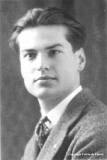
\includegraphics[width=\threefig]{\figdir/deFinetti.jpg}
%       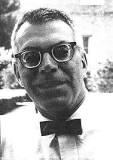
\includegraphics[width=\threefig]{\figdir/savage.jpg}
%       \caption{Bruno de Finetti (1906--1985) and L. ``Jimmie" Savage (1917--1971)}
%     \end{figure}
%   \end{itemize}
% \end{frame}

% \begin{frame}{Savage's axioms}
% \begin{itemize}
% \item Start with the triple $(\cS,\cZ,\cA\subset \cF(\cS, \cZ))$ as in \cite{Wal50}.
% \item Savage's idea is to list what we expect from a binary relation $\prec$ on $\cA\times \cA$ describing a decision maker's preferences.
% \end{itemize}
% \blank
% \blank
% \end{frame}

% \begin{frame}{Savage's axioms}
% \end{frame}

% \begin{frame}{Savage's axioms}
% \end{frame}

% \begin{frame}{A De Finetti theorem by Hewitt \& Savage}
%   \begin{block}{Theorem; see \citep[Theorem 1.49]{Sch12}}
%     Let $X_1,X_2,\dots$ be a sequence of exchangeable random variables on $\cX$, i.e.
%     $$
%     X_1,\dots,X_n \sim X_{\pi(1)},\dots, X_{\pi(n)}, \forall n, \forall \pi\in\frak S_n.
%     $$
%     Then there exists a probability distribution $\mu$ \un{on the set of probability measures $\mathcal P(\cX)$ on $\cX$} such that
%     $$
%     \mathbb P (X_1\in A_1, \dots, X_n\in A_n) = \int Q(A_1)\dots Q(A_n)\d\mu(Q).
%     $$
%     % Furthermore, for each $A$,
%     % $$
%     % Q(A) = \lim_{n\rightarrow\infty} \frac 1n\sum_{i=1}^n 1_A(X_i)\quad a.s.
%     % $$
%   \end{block}
%   \vfill
%   To a subjectivist, Savage's theorem says you should use SEU, and representation theorems like de Finetti's constrain your choice of $p$.
% \end{frame}

% % \begin{frame}{De Finetti's theorem and LDA}
% % \end{frame}

% % \begin{frame}{De Finetti's theorem and Bayesian nonparametrics}
% % \end{frame}

% \begin{frame}{Bonus: The Dirichlet process through de Finetti's theorem}

% \begin{block}{The Blackwell-McQueen urn scheme (aka the CRP)}
%   Start with an urn containing a single black ball with weight $\alpha$. Repeat: draw a ball from the urn with probability $\propto$ its weight. Then,
%   \begin{itemize}
%     \item If the ball is black, return it to the urn along with another ball of weight 1, with a \un{new color} sampled from some base measure $H$.
%     \item If the ball is colored, return it to the urn along with another ball of weight 1 of the \un{same color}.
%   \end{itemize}
%   Denote by $X_1, X_2, \dots$ the color of the ball added.
% \end{block}
% \begin{flushright}
%   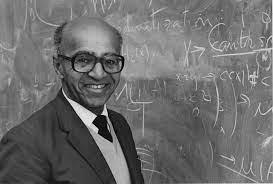
\includegraphics[width=\twofigminus]{Figures/blackwell.jpg}
% \end{flushright}
% \vfill
% % \begin{itemize}
% %   \item Exercise: show that $X_1,X_2,...$ are exchangeable.
% %   \item The corresponding prior $\mu$ on $\mathcal{P}(\cX)$ is the Dirichlet process with concentration $\alpha$ and base measure $H$.
% % \end{itemize}
% \end{frame}

% \begin{frame}{Pros and cons of the subjectivist viewpoint}
% \begin{itemize}
%   \item Axiomatic derivations are powerful, and shed light on what coherence requires. \un{In particular, coherence leads to SEU}.
%   \vfill
%   \item[\frownie] ... Yet all axiomatic systems have a bit that is difficult to swallow.
%   \vfill
%   \item Priors should be elicited by \un{expert knowledge}, and should be \emph{bona fide} probability distributions.
%   \vfill
%   \item Representation theorems can help design the joint distribution over states \citep{OrRo14}.
%   \vfill
%   \item Bayesian nonparametrics has revived the subjectivist viewpoint.
% \end{itemize}

% \end{frame}


\part{Implementing Bayesian machine learning}
    \chapterimage{chapter_head_1.pdf} % Chapter heading image
    \chapter{Markov chain Monte Carlo}
    Maximizing expected utility requires computing integrals. 
Numerical integration consists in finding $T$ nodes $x_t$ and weights $w_t$, such
that
$$
{\mathcal{E}_t(f)} \triangleq  \int f(x)\d\mu(x)  - \quad \sum_{t=1}^N w_t f(\theta_t) = o_{T\rightarrow \infty}(1), \quad \forall
f:\mathbb{R}^d\rightarrow\mathbb{R}\in\mathcal C,
$$
where $\mathcal C$ is a large class of functions.
Riemann-like (i.e., grid-based) integration leads to $\mathcal{E}_t(f) \sim \frac{\sqrt{d}}{T^{1/d}}$, so that grids become essentially useless beyond $d=3$.
Monte Carlo methods are randomized constructions of nodes and weights. 
Since $\mathcal{E}_T(f)$ is then random, statements on the error shall be with high probability, in expectation, about the asymtotic fluctuations, etc.

We shall see that Monte Carlo methods $(i)$ can accomodate settings where the target $\mu$ in \eqref{e:numerical_integration} is only available through the evaluation of a unnormalized density $\d\mu(x) = \pi(x)\d x = \pi_u(x)/Z\d x$, as is almost always the case in Bayesian learning; and that $(ii)$ some Monte Carlo methods have an error that scales only polynomially with the dimension of the support of the integrand.

\paragraph{References.} 
The reference book for basic Monte Carlo methods is \citep{RoCa04}. 
For theoretical results on MCMC, we refer to \citep[Chapters 5 to 7]{DoMoSt14}. 
For more recent methods, we shall refer to papers.
For demos of MCMC samplers, see \cfdemo.
Finally, we shall not cover deterministic alternatives to Monte Carlo methods in large dimension, see quasi-Monte Carlo methods \citep{DiPi10}.

\section{Basic Monte Carlo}

If we knew how to sample from $\pi$, we could take $x_t\sim\pi$ i.i.d., $w_t=1/T$.
Chebyshev's inequality would lead to
  $$ \mathbb{P}\left({\mathcal{E}_T(f)} \geq \alpha\frac{\sigma(f)}{\sqrt{T}} \right) \leq \frac{1}{\alpha^2}, \quad \forall \alpha>0,$$
  as soon as $\sigma(f)^2 := \mathbb{E}_{X\sim\pi} [f(X) - \int f(x)\pi(x)\d x]<+\infty$.

In practice, we never have access to a sampler of $\pi$, so we choose an instrumental distribution $q(x)\d x$, sample $x_t$ i.i.d. from $q$.
If we can evaluate $\pi$, then $w_t=\pi(x_t)/q(x_t)$ leads to an unbiased estimator called the \emph{importance sampling}. 
Its error can also be controlled by the Chebyshev inequality. 
But more often than not, we can only evaluate an unnormalized density $\pi_u$. 
An alternative is to then set $w_t\propto \pi_u(x_t)/q(x_t)$ and normalize the weights so that $\sum_t w_t=1$. 
This leads to the \emph{self-normalized importance sampling estimator}
$$
\widehat I_T^\text{NIS} = \frac{\sum_{t=1}^T \frac{\pi_u(\theta_t)}{q(\theta_t)} f(x_t)}{\sum_{t=1}^T \frac{\pi_u(\theta_t)}{q(\theta_t)}} \rightarrow \frac{\int f(x)\pi_u(x)\d x}{\int \pi_u(x)\d x} = \int f(x)\d x,
$$
where the convergence is almost sure (apply the strong law of large numbers to both the numerator and the denominator).
\begin{proposition}[CLT for NIS] The NIS estimator satisfies
   $$
   \sqrt{T} \left (\widehat I_T^\text{NIS} - \int f(x)\pi(x)\d x\right ) \rightarrow_d \cN(0,\sigma_{\text{NIS}}^2(f))
   $$
   where $f$ is such that
   $$
   \sigma_{\text{NIS}}^2(f) \triangleq TBC <\infty.
   $$
\end{proposition}
\begin{proof}
    See exercise sheet.
\end{proof}
Unfortunately, while NIS does accomodate unnormalized targets, it does not solve the curse of dimensionality: even when $\pi$ and $q$ are both Gaussian, only with different covariance matrices, one can show that 
$$
\log \sigma_{\text{NIS}}^2(f) = \Theta(d).
$$

\section{The Metropolis-Hastings algorithm}
Metropolis-Hastings (MH) is the achetypal MCMC algorithm, and is still the main building block of modern MCMC algorithms. 
The idea is to take the nodes as the truncated history of a Markov chain $(X_t)$, which we build so as to guarantee that $\mathcal{E}_T(f)\rightarrow 0$.
To see how to build $(X_t)$, remember first the law of large numbers for Markov chains. 

\begin{proposition}[LLN for Markov chains; see e.g. \cite{DoMoSt14}]
    Let $(X_t)_{t\in\mathbb N}$ be a Markov chain with Markov kernel $P$.
    If
    \begin{enumerate}
      \item There exists $\pi$ s.t. 
      $$
      \int \d\pi(x) P(x, B) = \pi(B).
      $$
      \item For any $A$ with $\pi(A)>0$, for any $\theta\in \Theta$,
      $$ 
      \mathbb{P}_{x} \left(\sum_{t=0}^\infty 1_{\theta_t\in A} = +\infty\right) = 1,
      $$
    \end{enumerate}
    then for any initial distribution $\mu_0$ of $X_0$, almost surely
    $$
    \frac{1}{T} \sum_{t=1}^T f(\theta_t) \rightarrow \int f\mathrm{d}\pi,
    $$
    where $f\in L^1(\pi)$. 
\end{proposition}
The first condition states that $\pi$ is an \emph{invariant distribution} of the chain: if $X_t\sim\pi$, then $X_{t+1}\sim\pi$. 
The second condition is called \emph{Harris recurrence}: starting from any $x$, i.e. $X_0\sim\delta_{x}$, then the chain returns an infinite number of times to $A$ almost surely, as soon as $A$ is charged by $\pi$. 
Intuitively, this makes sure that there is an infinity of nodes on $A$, so that the integral of $f$ on $A$ is accurately estimated.

\section{Gibbs sampling}

\section{Hamiltonian Monte Carlo}
We closely follow \cite{BoSa18}, who give a clear introduction to the ingredients of HMC.
To facilitate going back and forth between the notes and \citep{BoSa18}, we temporarily adopt their notational conventions: the variable over which we wish to integrate is $q\in\mathbb{R}^d$, while $x\in\cX$ denotes a generic variable, later taken to be $x=(p,q)$.
Note that vanilla HMC is limited to continuous variables.

\subsection{An abstract variant of Metropolis-Hastings}
\label{s:abstract_HMC}
Let $S$ be a linear involution of $\cX\subset\mathbb{R}^{2d}$, such that $\eta\circ S = \eta$ for some (possibly unnormalized) PDF $\eta$.
Let further $\Phi:\mathbb{R}^{2d}\rightarrow \mathbb{R}^{2d}$ be a $C^1$-diffeomorphism that is reversible w.r.t. to $S$, that is, $S\circ \Phi = \Phi^{-1}\circ S$.
Now let 
\begin{equation}
    \label{e:acceptance_probability_abstract_HMC}
    \alpha(x) \triangleq 1\wedge \frac{\eta(\Phi(x))}{\eta(x)} \vert\Phi'(x)\vert,
\end{equation}
and consider the Markov kernel
$$
P_{aHMC}(x,A) = \alpha(x) 1_{\Phi(x)\in A} + (1-\alpha(x))1_{S(x)\in A}.
$$
Algorithmically, this ``abstract" HMC kernel corresponds to accepting $\Phi(x)$ with probability $\alpha(x)$, and otherwise setting the new Markov state to $S(x)$.
\begin{proposition}
\label{p:invariance_abstract_HMC}
$P_{aHMC}$ leaves $\eta$ invariant.
\end{proposition}
\begin{proof}
    Left as an exercise.
\end{proof}

\subsection{An augmented target}
Consider the PDF on $\mathbb{R}^{2d}$ defined by $\tpi(q,p) = \frac12 \cN(p\vert 0, M) \times \pi(q)$. 
Clearly, the $p$-marginal is Gaussian, while the $q$-marginal is $\pi$. 
If we manage to obtain an MCMC chain for $\tpi$, i.e. a chain with a Markov kernel that leaves $\tpi$ invariant, then simply discarding the $p$-component of every realization will yield a chain that is invariant w.r.t. $\pi$. 
This is an example of \emph{augmentation} of the state space: unlike for the collapsed Gibbs sampling of Section~\ref{s:collapsed_gibbs}, we augment the dimensionality of the problem in the hope to make sampling easier. 
Our hope is justified here by the fact that we know how to efficiently move in $\mathbb{R}^{2d}$ along the level lines of the augmented density $\tpi$: this is were Hamiltonian dynamics come into play.

\subsection{Hamiltonian dynamics}
\label{s:hamiltonian_dynamics}
Let $H(q,p) = \log\tpi(q,p)$, and consider the differential equation 
\begin{equation}
    \label{e:differential_equation}
    \frac{\d}{\d t} \begin{pmatrix} x\\p \end{pmatrix} = J \nabla H(q,p), \quad\text{ where } J=\begin{pmatrix} 0_d & -I_d \\ I_d & 0_d \end{pmatrix}.
\end{equation} 
In particular, if $\nabla H$ is Lipschitz, which we shall always assume in this section, the Cauchy-Lipschitz theorem yields a unique solution to \eqref{e:differential_equation} passing through $(q_0,p_0)$ at $t=0$, which we denote by $t\mapsto \phi_t(q_0,p_0)$.
We shall further assume that $\phi_t$ is well defined for all $t$, and call $\phi_t$ the \emph{Hamiltonian flow}. 
By definition, the Hamiltonian flow preserves the Hamiltonian, since
$$
\frac{\d}{\d t} H(\phi_t(q_0,p_0)) = \nabla H(\phi_t(q_0,p_0))^T J \nabla H(\phi_t(q_0,p_0)) = 0,
$$
$J$ being skew-symmetric.
In other words, the flow $\phi_t$ follows level lines of $H$.

\subsection{Ideal HMC and numerical HMC}
The ideal HMC is the concatenation of two kernels. 
Given $(q_n,p_n)$, first resample $p$ from its conditional under $\tpi$; i.e. $p'\sim \cN(0,M)$. 
This obviously leaves $\tpi$ invariant, as in Gibbs sampling. 
Then set $(q_{n+1}, p_{n+1}) = \phi_T(q_n,p')$.
In words, one step of the corresponding Markov chain consists of sampling a random momentum variable from the corresponding conditional, and then following the Hamiltonian flow $\phi_t$ up to time $T>0$.
Note that, unlike Gibbs sampling, this second step changes both variables.

One can formulate the intuition that, since the second step just follows a level line of $H$, the ideal HMC kernel leaves $\tpi$ invariant. This is indeed the case \citep{BoSa18}, but since $\phi_t$ is usually not available in closed form, the ideal HMC kernel cannot be implemented, and we will skip the proof of its invariance. 

In practice, one has to approximate the Hamiltonian flow $\phi_t$, and there is a large literature in numerical analysis on the subject, with integrators showcasing many interesting properties.
In terms of notation, denote by $h$ a stepsize parameter, and $n=\lfloor T/h\rfloor$, so that we think of the numerical integrator $\psi_h^n(x,p)$ as an approximation to $\phi_T(x,p)$.
There exists numerical integrators $\phi_h^n$ that are $(i)$ $C^1$ diffeomorphisms, $(ii)$ are reversible w.r.t. to momentum flip, and are volume-preserving, i.e. $\vert \det (\psi_h^n)'(q,p)\vert = 1$.
Since the momentum flip preserves $\tpi$, we can replace the second step of the ideal HMC algorithm by the abstract HMC algorithm of Section~\ref{s:abstract_HMC}, with $\eta=\tpi$, $\Phi=\phi_h^n$ and $S$ the momentum flip. 
Because the numerical integrator is volume-preserving, the acceptance probability becomes suprisingly simple, as 
$$ 
\alpha_{HMC}((q,p),(q',p')) = 1\wedge \e^{-H(q,p)-H(q',p')}.
$$
Intuitively, the acceptance step compensates for the fact that we did not exactly follow the level lines of $H$. 

One common numerical integrator satisfying all the required properties is the leapfrog (aka velocity Verlet in \citep{BoSa18}) integrator defined as $\psi_h^n = \psi_h \circ \dots \psi_h$, where $(p',q') = \psi_h(p,q)$ is defined by
\begin{align*}
    p_{1/2} &= p + \frac{h}{2}\nabla \log \pi(q)\\
    q' &= a+hM^{-1}p_{1/2}\\
    p' &= p_{1/2} + \frac{h}{2} \nabla \log\pi (q');
\end{align*}
see \citep[Section 3]{BoSa18} for more information, and \cfdemo for an interactive demo.

\subsection{On the ergodicity of HMC}

\subsection{An ubiquitous variant: NUTS}
NUTS for auto-tuning, etc.

\section{MCMC practice: convergence diagnostics}
Convergence diagnostics. Discuss the output of pymc.


    \chapter{Variational Bayes}
    %!TEX root=./main.tex

While Monte Carlo methods are randomized numerical quadratures, \emph{variational Bayes} (VB) stands for finding an approximation to the target distribution within some prespecified set $\mathcal Q$ of distributions.
This is done by minimizing some notion of distance between the target $\pi$ and the so-called variational approximation $q\in\mathcal Q$.
For instance, a common choice is to solve
\begin{equation}
q^\star \in \arg\min_{q\in\mathcal Q} \text{KL}(q, \pi) := \mathbb E_q \log \frac{q(\theta)}{\pi(\theta)} = \int q(\theta) \log \frac{q(\theta)}{\pi(\theta)} \d\theta,
\label{e:VB}
\end{equation}
where $\pi$ and $q$ are PDFs w.r.t. some common measure $\d\theta$.
Once \eqref{e:VB} has been solved, one can either use the resulting $q^\star$ as a plug-in replacement for the target $\pi$, or, say, use $q^\star(\theta)\d\theta$ as a proposal distribution in importance sampling.

Compared to MCMC, the big plus of VB is that some modification of the optimization problem \eqref{e:VB} can often be implemented in large-scale settings where either the number of data items or the dimension of the problem are large, e.g. in deep learning.
The major downside of VB is the difficulty to provide theoretical guarantees on its results.
One reason for this is that the distance to minimize, such as the reverse KL divergence in \eqref{e:VB}, is often chosen for computational convenience rather than for its guarantees on integrating functions of interest.
Another reason is that approximating complex target distributions requires a large set $\mathcal Q$ of variational approximations, which usually makes \eqref{e:VB} a difficult optimization problem that has to be further modified before an efficient implementation is possible.

\section{The evidence lower bound (ELBO)}
Remember that the density $\pi$ is often known only though the evaluation of an unnormalized version $\pi_u$, i.e., $\pi_u(\theta) = Z\pi(\theta), \forall \theta$.
If we are to carry out \eqref{e:VB}, we thus need to know how to express $\text{KL}(q,\pi)$ using only $\pi_u$.

\begin{lemma}
Let $J(q) := \int q(\theta) \log \frac{q(\theta)}{\pi_u(\theta)}\d\theta$.
Then
\begin{equation}
J(q) = \text{KL}(q, \pi) - \log Z.
\label{e:preELBO}
\end{equation}
\end{lemma}

\begin{proof}
  Left as an exercise.
\end{proof}

Two remarks are in order.
First, since $Z$ does not depend on $q$, the optimization problem in \eqref{e:VB} is equivalent to $\min J(q)$.
Letting $ L(q) = -J(q)$, \eqref{e:VB} is further equivalent to $\max L(q)$.
Second and the nonnegativity of the KL divergence implies that
\begin{equation}
L(q) \leq \log Z.
\label{e:ELBO}
\end{equation}
In Bayesian inference,
$$
\pi_u(\theta) = p(y_{1:N}\vert\theta) p(\theta),
$$
so that $Z=p(y_{1:N})$.
Furthermore, \eqref{e:ELBO} says that $L(q)$ is \emph{a lower bound for the (logarithm of the) evidence}, shortened in ELBO.
Most VB algorithms in the literature are cast as maximizing the ELBO.

\section{Mean-field inference}
The most common variational family is the so-called \emph{mean-field approximation}.
If you need to approximate a posterior over parameters $\theta\in\mathbb{R}^d$ and latent variables $z_1,\dots,z_N$, this means taking
\begin{equation}
  \label{e:mean_field}
  \mathcal Q = \left\{\theta\mapsto \prod_{d=1}^D q_d(\theta_d) \prod_{i=1}^N q_i(z_i)\right\}.
\end{equation}
In other words, we approximate $\pi$ with a separable PDF.
Note that \eqref{e:mean_field} only specifies the structure of the variational approximations.
This is enough to derive the abstract form of the VB updates, which we do in the remainder of this section.
In practice, though we further make explicit parametric choices for the individual factors, as we shall see in Section~\ref{s:VB_for_LDA}.

The whole motivation of the mean-field variational family is that if your target has simple conditionals, coordinate-wise optimization of the ELBO is easy.
Indeed, write $x=(\theta,z) \in \mathbb{R}^p$ and let $1\leq i\leq p$. Writing $q(x) = q_i(x_i)q_{\setminus i}(x_{\setminus i})$, and keeping track only of the additive terms that depend on $q_i$, it comes
\begin{align*}
L(q)
&= \iint  q_i(x_i)q_{\setminus i}(x_{\setminus i}) \left[\log \pi_u(x) - \left( \log q_i(x_i) + \log q_{\setminus i}(x_{\setminus i}) \right)\right] \d x_i \d x_{\setminus i}\\
&\propto \int q_i(x_i) \left[ \int q_{\setminus i}(x_{\setminus i}) \log \pi_u(x) \d x_{\setminus i}\right] d x_i- \int q_i(x_i)\log q_i(x_i) \d x_i\\
&= - KL(q_i,\phi_i),
\end{align*}
where
\begin{equation}
  \label{e:intermediate_distribution}
  \phi_i(x_i) = \exp \left[\int q_{\setminus i}(x_{\setminus i}) \log \pi_u(x) \d x_{\setminus i}\right]
\end{equation}
is an unnormalized PDF. By a fundamental property of the KL, the ELBO $L$ is thus maximized by setting $q_i\propto \phi_i$.
The bottleneck is thus to be able to compute $\phi_i$ in \eqref{e:intermediate_distribution}.
Like in deriving conditionals in Gibbs sampling, this is the part where conjugate distributions play a role.
In practice, the choice of $\mathcal Q$ is often made so that this step is easy, as we shall see in Section~\ref{s:VB_for_LDA}.

Finally, note that taking the variational family to be \eqref{e:mean_field} is akin to assuming independence of all variables under the posterior.
Combined with the fact that reverse KL \eqref{e:VB} penalizes $q^\star$ putting a lot of mass where $\pi$ does not, this often implies a gross underestimation of the support of the target (and thus of posterior uncertainty), along with the built-in ignorance of posterior correlations; see Figure~\ref{}.
While separability makes algorithmic derivations easier, we thus usually rather aim for ``as separable as required by computation".
In other words, if, for modeling reasons, you believe that there is correlation under $\pi$ of some subset of the variables, say $x_i, i\in I$, you should try to keep these variables correlated in your variational approximation, by rather defining
$$
\mathcal Q = \left\{\theta\mapsto q_I(x_I) \prod_{i \notin I} q_i(x_i) \right\},
$$
for some nonseparable $q_I$.
\cite[Chapter 23]{Mur12} calls this \emph{structured mean-field}.

\subsection{Mean-field VB for LDA}
\label{s:VB_for_LDA}
Recall the latent Dirichlet allocation model from Section~\ref{s:Gibbs_for_LDA}, for which
\begin{align}
\log &p(y, z, \pi, B)\\
&=\sum_{i=1}^N \left[\log p(\pi_i\vert \alpha) + \sum_{\ell=1}^{L_i} \Big(\un{\log p(z_{i\ell}\vert\pi_i)} + \unn{\log p(y_{i\ell}\vert z_{i\ell}, B)\Big)}\right] + \unnnn{p(B\vert \gamma)}\nonumber\\
&\propto \sum_{i=1}^N \left[\sum_{k=1}^K \alpha_k \log \pi_{ik} + \sum_{\ell=1}^{L_i} \left(\un{\sum_{k=1}^K 1_{z_{i\ell}=k}\log\pi_{_{ik}}} + \unn{\sum_{v=1}^V \sum_{k=1}^K 1_{y_{i\ell}=v}1_{z_{i\ell}=k} \log b_{kv}}\right)\right] \nonumber\\
&~~~~~+ \unnnn{\sum_{k=1}^K \sum_{v=1}^V \gamma_v\log b_{kv}}. \label{e:LDA_joint}
\end{align}
We want to fit a mean-field approximation
$$
\mathcal Q = \left\{ \prod_{i=1}^N \left[\text{Dir}(\pi_i\vert\widetilde{\pi_i}) \prod_{\ell=1}^{L_i} \text{Cat}(z_{i\ell}\vert\widetilde{z}_{i\ell}) \right] \prod_{k=1}^K \text{Dir}(B_{k:}\vert \widetilde{B}_{k:}) \right\}.
$$
Tilded variables parametrize the variational approximation $q$, and optimizing over $q$ will thus be implemented as an optimization over these parameters.
As we shall see, the Dirichlet distributions are chosen to make the following computations easy thanks to conjugacy.

To implement VB, we need to compute \eqref{e:intermediate_distribution} for every coordinate, that is, we need to integrate the log joint distribution \eqref{e:LDA_joint} with respect to all variables but one, for every choice of that singled out variable.

\paragraph{Singling out $\pi_i$.}
We start by singling out $\pi_i\in \Delta_K$ for some $1\leq i \leq N$, denoting the corresponding expectation by $\mathbb E_{\setminus \pi_i}$.
We are confident that we shall be able to identify the functional form (and thus the normalization constant) of the resulting distribution, and thus we do not keep track of additive variable that do not imply $\pi_i$.
This yields
\begin{align*}
\mathbb{E}_{\setminus \pi_i} \log p(y,z,\pi, B) &\propto \sum_{k=1}^K \alpha_k \log \pi_{ik} + \sum_{\ell=1}^{L_i} \mathbb{E}_{z_{i\ell}}\un{\sum_{k=1}^K  1_{z_{i\ell}=k}\log\pi_{_{ik}}}\\
&= \sum_{k=1}^K \alpha_k \log \pi_{ik} + \sum_{\ell=1}^{L_i} \un{\sum_{k=1}^K \widetilde{z}_{i\ell k}\log\pi_{_{ik}}}
\end{align*}
and we recognize the log PDF of a Dirichlet distribution in $\pi_i$, with parameters
$$
\widetilde\pi_i \triangleq \left( \alpha_k + \sum_{\ell=1}^{L_i} \widetilde{z}_{i\ell k}  \right)_{1\leq k\leq K}.
$$

\paragraph{Singling out $z_{i\ell}$.}
To compute $\mathbb{E}_{\setminus z_{i\ell}} \log p(y,z,\pi, B)$, we need to be able to compute expectation of log weights w.r.t. a Dirichlet distribution.
\begin{lemma}
Let $\Psi(\cdot) := \Gamma'(\cdot)/\Gamma(\cdot)$ be the digamma function.
Let $\widetilde\eta\in \Delta_M$ be a probability distribution over $\{1,\dots, M\}$.
Then, for $m\in \{1,\dots, M\}$,
$$
  \mathbb{E}_{\text{Dir}(\eta\vert\widetilde\eta)} \log \eta_m = \Psi(\widetilde\eta_m) - \Psi(\Vert \widetilde\eta\Vert_1) \triangleq \Psi_m(\widetilde{\eta}).
$$
\end{lemma}
\begin{proof}
  Left as an exercise.
\end{proof}

Now we derive
\begin{align*}
  \mathbb{E}_{\setminus z_{i\ell}} \log p(y,z,\pi, B)
    &\propto  \un{\sum_{k=1}^K  1_{z_{i\ell}=k} \mathbb{E}_{\pi_i}\log\pi_{_{ik}}}
    + \unn{\sum_{v=1}^V \sum_{k=1}^K 1_{y_{i\ell}=v} 1_{z_{i\ell}=k} \mathbb{E}_{B_{k:}}\log b_{kv} }\\
    &=  \un{\sum_{k=1}^K  1_{z_{i\ell}=k} \Psi_k(\widetilde\pi_{i})}
    + \unn{\sum_{v=1}^V \sum_{k=1}^K 1_{y_{i\ell}=v} 1_{z_{i\ell}=k} \Psi_v(\widetilde{B}_{k:}) }
\end{align*}
We recognize a categorical distribution with parameters
$$
\widetilde{z}_{i\ell} \propto \left( \exp\left[\Psi_k(\widetilde\pi_{i}) +  \Psi_{y_{i\ell}}(\widetilde{B}_{k:})\right]\right)_{1\leq k \leq K}.
$$
Once again, the normalization constant can be guessed after doing the computation, since necessarily
$$
  \widetilde{z}_{i\ell} =
    \left(
      \frac{\exp\left[\Psi_k(\widetilde\pi_{i}) +  \Psi_{y_{i\ell}}(\widetilde{B}_{k:})\right]}
      {\sum_{k=1}^K \exp\left[\Psi_k(\widetilde\pi_{i}) +  \Psi_{y_{i\ell}}(\widetilde{B}_{k:})\right]}
    \right)_{1\leq k \leq K}.
$$

\paragraph{Singling out $B_{k:}$}
In the same vein,
\begin{align*}
  \mathbb{E}_{\setminus B_{k:}} \log p(y,z,\pi, B)
    &\propto \unn{\sum_{i=1}^N\sum_{\ell=1}^{L_i}\sum_{v=1}^V 1_{y_{i\ell}=v} \mathbb{E}_{z_{i\ell}} 1_{z_{i\ell}=k} \log b_{kv} } + \unnnn{\sum_{v=1}^V \gamma_v\log b_{kv}}
\end{align*}
and we recognize a Dirichlet with parameters
$$
\widetilde{B}_{k:} \triangleq \left (\gamma_v + \sum_{i=1}^N\sum_{\ell=1}^{L_i} 1_{y_{i\ell}=v}\widetilde{z_{i\ell k}} \right)_{1\leq v \leq V}.
$$
This concludes the derivation of VB for LDA.

\subsection{Mean-field VB for marginal LDA}
As an exercise, derive the updates for the marginalized LDA model of Section~\ref{s:marginal_LDA}; see \cite[Chapter 27.3]{Mur12} for the solution.

\subsection{VB generalizes the EM algorithm}
TBC

\section{Gradient-based algorithms}
An alternate approach to finding a simple $\mathcal Q$ leading to closed-form updates is to directly run a gradient algorithm on the ELBO \eqref{e:ELBO}.
Take $\mathcal{Q} = \{q(\cdot\vert\phi), \phi \in\Phi\}$, where for all $x$, $\phi\mapsto q(x\vert\phi)$ is differentiable.
Then, assuming the necessary regularity conditions, \cite{PaBlJo12} note that gradient of the ELBO can be rewritten using the so-called \emph{score function trick} as
\begin{align*}
\nabla_\phi L(q) 
&= \nabla_\phi \mathbb{E}_{x\sim q(\cdot\vert\phi)} \log \frac{\pi_u(x)}{q(x\vert\phi)}\\
&= \int \log \pi_u(x) \nabla_\phi q(x\vert\phi) \d x + \nabla_\phi H[q(\cdot\vert\phi)].\\
&= \mathbb E_{{x\sim q(\cdot\vert\phi)}} \left [\log \pi_u(x) \nabla_\phi \log q(x\vert\phi) \right ] + \nabla_\phi H[q(\cdot\vert\phi)].
\end{align*}
The first term can be estimated by vanilla Monte Carlo. 
The entropy term can usually be differentiated in closed form; if not, it can be estimated by vanilla Monte Carlo as well. 
Overall, we can plug an unbiased estimator of the gradient of the ELBO in any stochastic gradient algorithm. 
More often than not, the ELBO as a function of $\phi$ is not convex, though, and one has to be happy with searching for local optima. 
Moreover, vanilla Monte Carlo estimators of \eqref{e:gradient_of_the_ELBO} have been reported to have high variance even in simple models \cite{PaBlJo12}. 

Variance reduction for ELBO gradients has been a field of active research.
\cite{PaBlJo12} propose to use control variates, while \cite{KiWe14} and a large body of follow-up work propose \emph{reparametrization tricks} that work as follows. 
Assume that there exists a (deterministic) smooth and invertible function $f$ such that $f(\epsilon,\phi)\sim q(\cdot\vert\phi)$ whenever $\epsilon\sim p(\epsilon)$, with $\epsilon$ easy to sample.
Now rewrite 
\begin{align*}
  \nabla_\phi L(q) 
  &= \nabla_\phi \mathbb{E}_{\epsilon\sim p} \log \frac{\pi_u(f(\epsilon,\phi))}{q(f(\epsilon,\phi)\vert\phi)}+ \nabla_\phi H[q(\cdot\vert\phi)].
\end{align*}
This time the gradient can be passed under the integral in the first term, without relying on the score function trick, and we obtain
\begin{align*}
  \nabla_\phi L(q) 
  &= \mathbb{E}_{\epsilon\sim p} \nabla_\phi \log \pi_u(f(\epsilon,\phi)) + \nabla_\phi H[q(\cdot\vert\phi)].
\end{align*}
As long as we can compute gradients of $\log\pi_u$, we can compute the gradient in the expectation using the chain rule. 
This suggests a second vanilla Monte Carlo estimator, drawing $\epsilon_i\sim p$ i.i.d. 
In practice, the resulting estimator has been found to have much lower variance \citep{ReMoWi14}, like in variational auto-encoders \citep{KiWe14}. 
I haven't seen a completely convincing explanation why and when variance reduction happens with the reparametrization trick in general, though.  
Finally, note that we again assumed that the entropy of $q$ could be differentiated in closed form, but the entropy term can also be treatead using the reparametrization trick if needed. 

\subsection{VB for deep networks}
% Include IS with VAEs as in Jordan et al.
One of the hot applications of gradient-based VB is for Bayesian deep learning, which has generated a huge literature in a short amount of time; see e.g. recent NeurIPS tutorials and workshops for pointers.  
For instance, \cite{BCKW15} proceed as follows.
We consider networks as generative models, so consider the softmax (classification) or squared (regression) loss.
A network thus corresponds to a likelihood $p(\mathbf{y}\vert w)$.
We take a prior $p(w)$ for the weights, and want to fit $q(w\vert\phi)$ to the posterior $\pi(w) \propto p(\mathbf{y}\vert w)p(w) = \pi_u(w)$.
The gradient of the reparametrized ELBO writes
\begin{align*}
\nabla_\phi L(q(\cdot\vert\phi)) &= \mathbb E_\epsilon \nabla_\phi \log \frac{\pi_u(f(\epsilon,\phi))}{q(f(\epsilon,\phi)\vert\phi)}\\
&\approx \frac{1}{N_\epsilon} \sum_{i=1}^{N_\epsilon} \nabla_\phi \log \frac{\pi_u(f(\epsilon_i,\phi))}{q(f(\epsilon_i,\phi)\vert\phi)}.
\end{align*}
Now notice that $\log\pi_u(w) = \log p(w) + \sum_{i=1}^{N_y} \log p(y_i\vert w)$, so that one can further uniformly draw (with or without replacement) a minibatch of data points $B$, and further obtain an unbiased estimator 
\begin{align*}
\nabla_\phi L(q(\cdot\vert\phi)) &\approx \frac{N_y}{N_\epsilon \vert B\vert} \sum_{i=1}^{N_\epsilon} \sum_{y\in B} \nabla_\phi \left [ \frac{1}{N_y}\log p(f(\epsilon_i,\phi)) + \log p(y\vert f(\epsilon_i,\phi)) - \log q(f(\epsilon_i,\phi)\vert\phi) \right ].\\
\end{align*}
Note that following \cite{BCKW15}, we do not assume that the entropy can be differentiated in closed form, but the method applies \emph{mutatis mutandis}. 
Note also that it is not obvious that replacing the entropy by its closed-form would reduce the variance of the estimator.

Now the key argument is that the gradient inside the sum can be computed using the chain rule, backprogagation, and the (assumed known) gradient of $q$.
As an example, assume $w\in\mathbb{R}^d$, $\phi=(\mu,\sigma)\in\mathbb{R}^{d+1}$, so that $f(\phi,\epsilon) = \mu + \sigma \epsilon \sim \mathcal{N}(\mu, \sigma I_d)$. 
For $y\in B$, Let $F(w) = \log p(y\vert w) + \log p(w)$. 
The gradient of $F$ is provided by backpropagation. 
Now the chain rule yields
\begin{align*}
  \nabla_\phi (F(f(\epsilon, \cdot))(\phi_0) &= J_{f(\epsilon,\cdot)}(\phi_0)^T \nabla F (f(\epsilon, \phi_0))\\
  &= \begin{pmatrix} I_d & \epsilon \\\end{pmatrix}^T \nabla F (f(\epsilon, \phi_0)).
\end{align*}

\section{Theoretical guarantees}

\section{Alternatives to the KL divergence}


\part{Nonparametric Bayes}
    \chapter{Random functions: Gaussian processes}
    \chapter{Random probability measures: Dirichlet processes and the like}
    \chapter{Asymptotic frequentist properties}

\part{Bayesian deep learning}
    \chapter{Bayesian neural networks}
    \chapter{Modern questions}

\chapter*{Bibliography}

% Bibliography
\addcontentsline{toc}{chapter}{\textcolor{ocre}{Bibliography}}
\printbibliography[heading=bibempty]

% Index
\cleardoublepage % Make sure the index starts on an odd (right side) page
\phantomsection
\setlength{\columnsep}{0.75cm} % Space between the 2 columns of the index
\addcontentsline{toc}{chapter}{\textcolor{ocre}{Index}} % Add an Index heading to the table of contents
\printindex % Output the index

\end{document}
